\clearpage

\section{Fitter performance. Study of residuals.}
\label{app:fitter_performance}

The fitter performance has been evaluated for different configurations: oscillation points, number of POT, levels 
of throwing systematics and fitters were varied. Residual distributions (best fit value - input value)  are 
presented in this section. For each study, 1000 toy datasets were created and fitted using MINUIT 
(MIGRAD), as explained in Sec.\ \ref{sec:neutrino_oscillation_fitting}. Table \ref{tab:osc_points} shows the true input values of the 
oscillation parameters for the different oscillation points studied. 

\begin{table}[htb]
\centering
\begin{tabular}{| c | c  c  c  c  c |}
\hline
Oscillation point &   $|\Delta m^2|$ (eV$^{2}$/c$^{4}$) & sin$^2\theta_{23}$ & sin$^2\theta_{13}$  & $\delta_{CP}$ & Mass Hierarchy \\
\hline
0  & 2.36 & 0.5 & 0.025 & 0 & NH\\
\hline
1  & 2.36 & 0.38 & 0.025 & 0 & NH\\
\hline
2  & 2.36 & 0.62 & 0.025 & 0 & NH\\
\hline
3  & 2.36 & 0.5 & 0.015 & 0 & NH\\
\hline
4  & 2.36 & 0.5 & 0.035 & 0 & NH\\
\hline
5  & 2.36 & 0.5 & 0.025 & $-\frac{\pi}{2}$ & NH\\
\hline
6  & 2.36 & 0.5 & 0.025 & $\frac{\pi}{2}$ & NH \\
\hline
7  & 2.2 & 0.5 & 0.025 & 0 & NH \\
\hline
8  & 2.8 & 0.5 & 0.025 & 0 & NH \\
\hline
9  & 2.36 & 0.5 & 0.025 & 0 & IH\\
\hline
\end{tabular}
\caption{
  True input values for the different oscillation points used in the study of fitter performance.
}
\label{tab:osc_points}
\end{table}


\subsection{'4 + 0' fit}

Figs. \ref{fig:residuals_40_first} - \ref{fig:residuals_40_last} show the distribution of residuals of the four 
oscillation parameters for each set described in table \ref{tab:osc_points} at $3.010 \times 10^{20}$ POT.
The distribution of residuals for $\delta_{CP}$ should not be taken into account due to the insensitivity to this parameter at current POT. 
A pileup similar to the one observed at maximal  mixing $sin^{2}(2\theta_{23}) = 1.0$ in the stand-alone disappearance 
analysis is now appearing at the center of symmetry of the P($\nu_{\mu}\rightarrow\nu_{\mu}$) curve,
which corresponds with the maximal disappearance (the difference between $sin^{2}(\theta_{23})$ values for maximal disappearance and
maximal mixing is explained in Sec. \ref{app:symmetry}).
This pile-up is reduced when the input value for $sin^{2}(\theta_{23})$ is far from 0.5 
(see figures  \ref{fig:residuals_40_point1} and  \ref{fig:residuals_40_point2}) and disappears if the 
POT is increased, as shown in figure \ref{fig:residuals_40_point1_x100}.
In general there are no unexpected features.

\clearpage

\begin{figure*}[htb]
\begin{minipage}[t]{0.5\linewidth}
\center
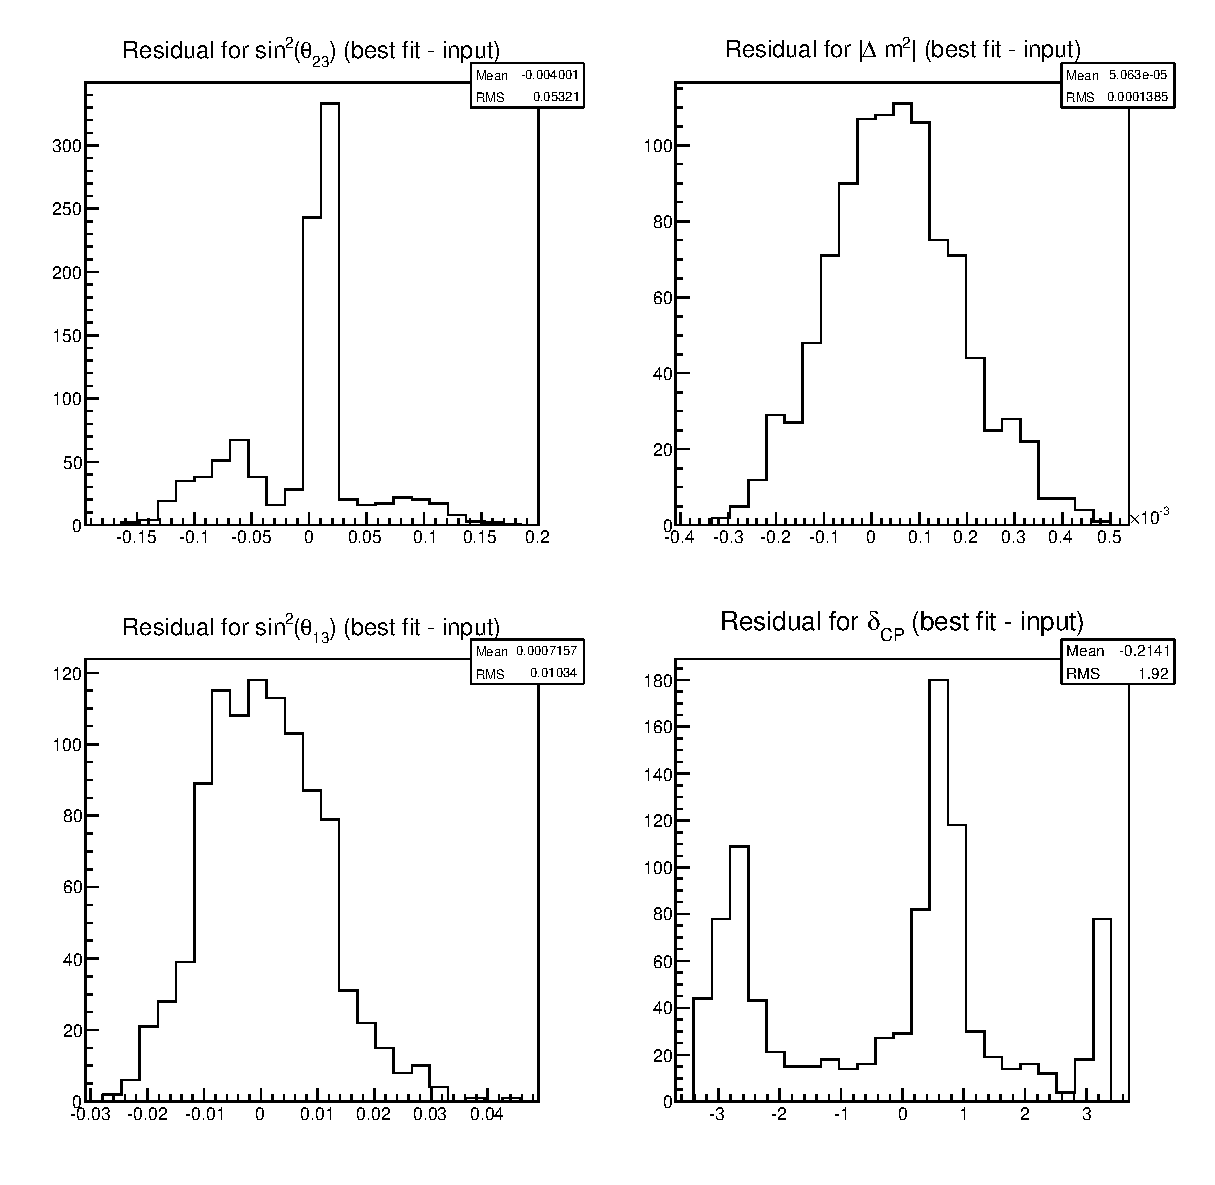
\includegraphics[width=18pc]{images/appendix/fitter_performance/Osc_residuals_nosyst_point0.eps}
\caption{
	Distribution of residuals of the four oscillation parameters in the '4 + 0' fit for oscillation point \# 0. 
 }
\label{fig:residuals_40_first}
\end{minipage}
\hspace{0.02\linewidth}
\begin{minipage}[t]{0.5\linewidth}
\center
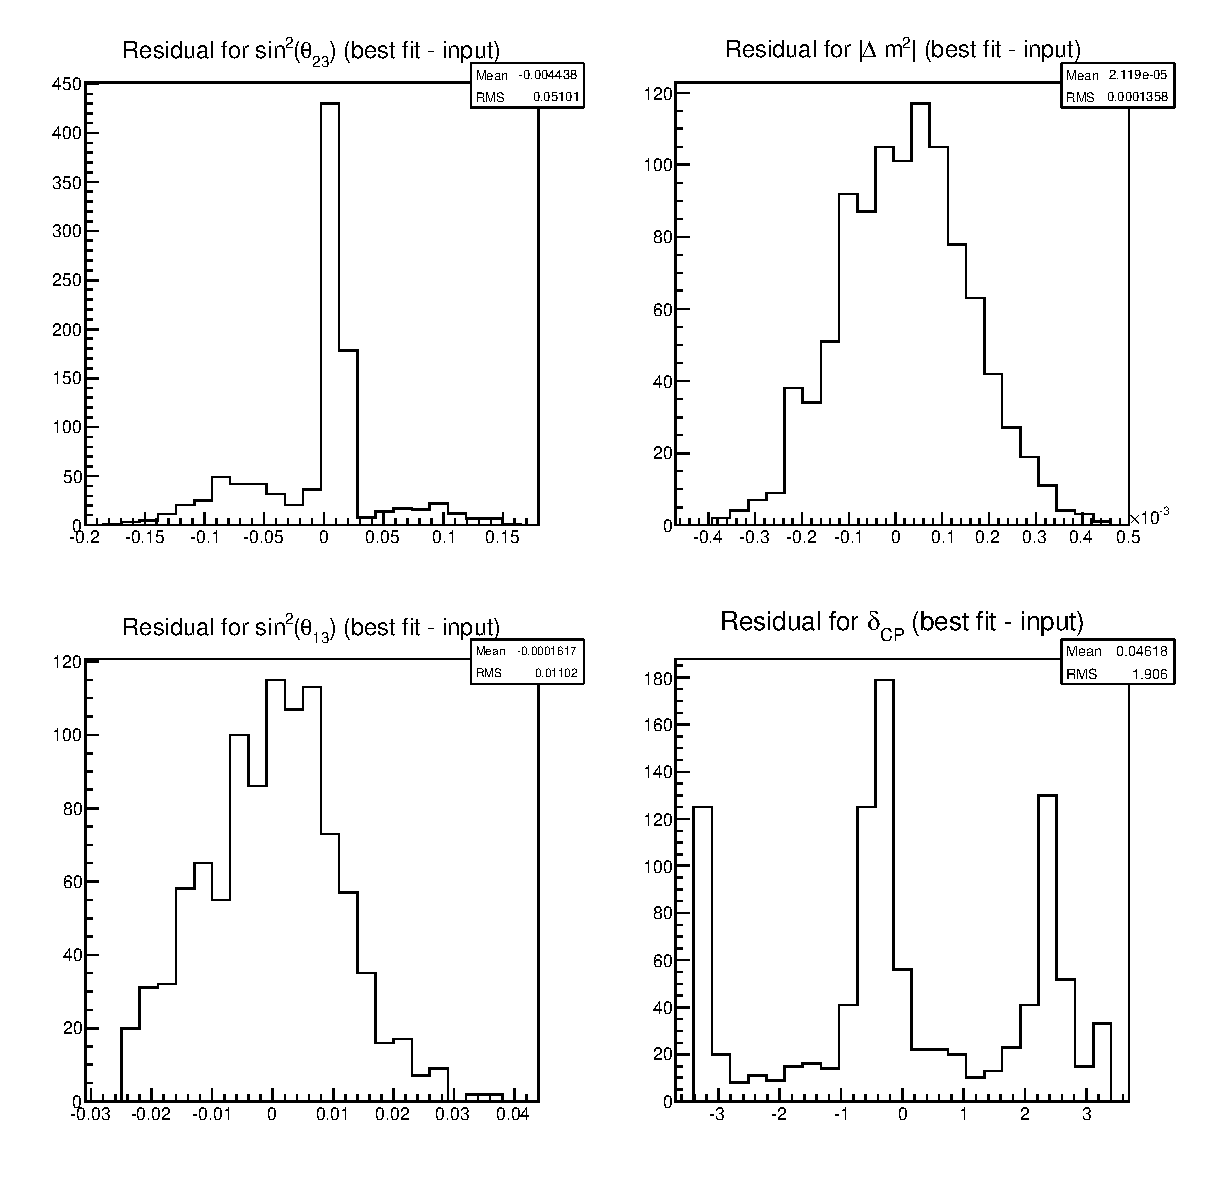
\includegraphics[width=18pc]{images/appendix/fitter_performance/Osc_residuals_nosyst_point9.eps}
\caption{
	Distribution of residuals of the four oscillation parameters in the '4 + 0' fit for oscillation point \# 9. 
 }
\end{minipage}

\end{figure*}


\begin{figure*}[htb]
\begin{minipage}[t]{0.5\linewidth}
\center
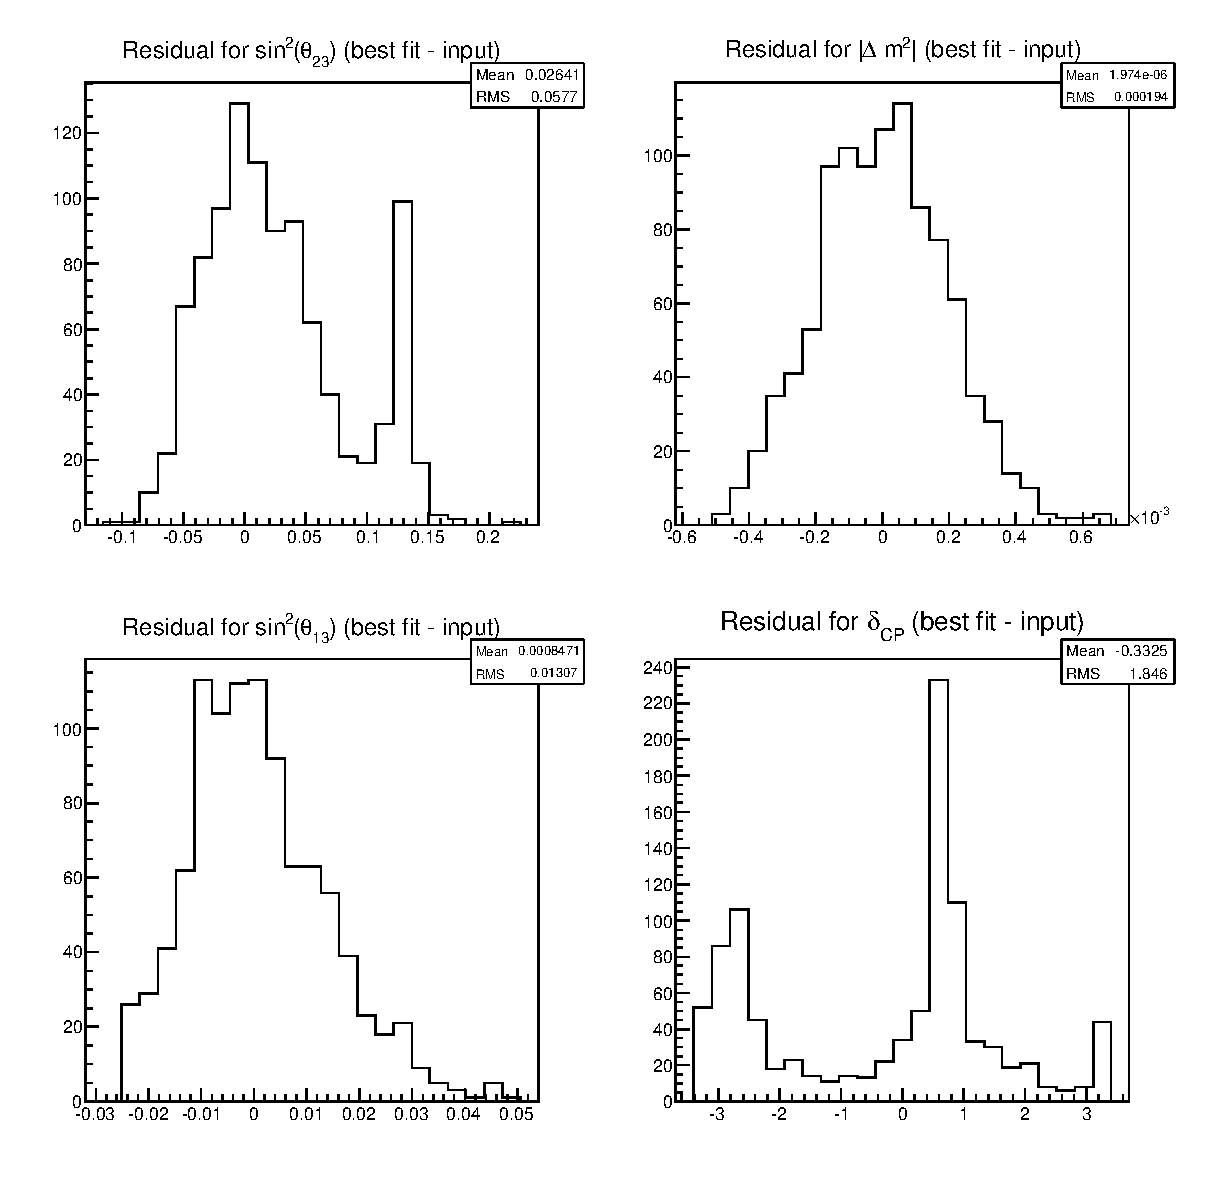
\includegraphics[width=18pc]{images/appendix/fitter_performance/Osc_residuals_nosyst_point1.eps}
\caption{
	Distribution of residuals of the four oscillation parameters in the '4 + 0' fit for oscillation point \# 1. 
 }
\label{fig:residuals_40_point1}
\end{minipage}
\hspace{0.02\linewidth}
\begin{minipage}[t]{0.5\linewidth}
\center
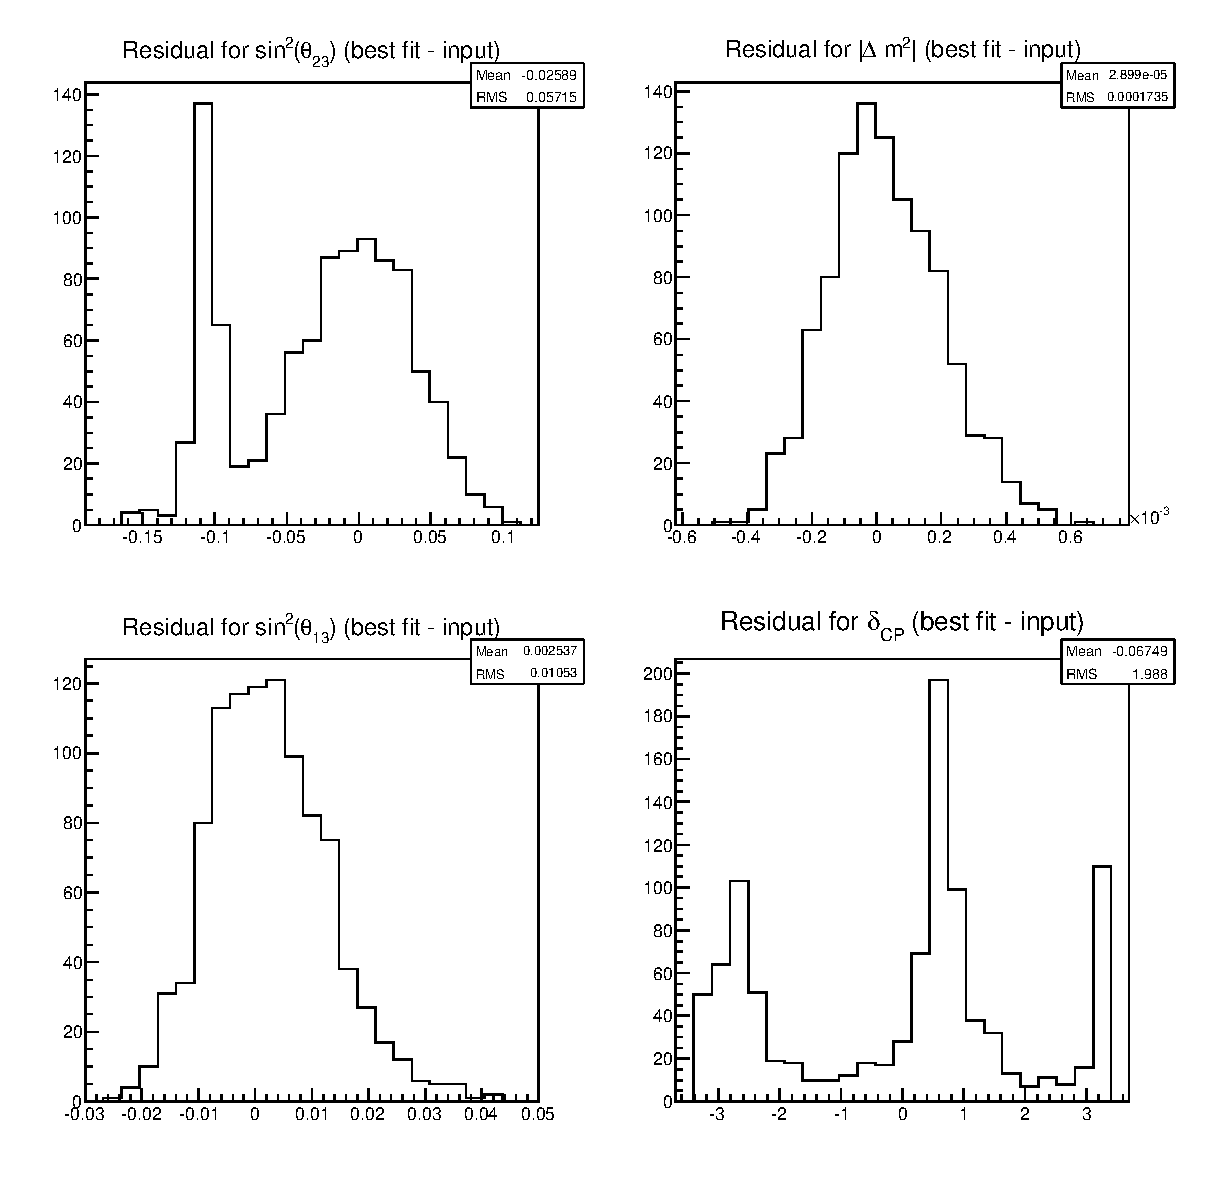
\includegraphics[width=18pc]{images/appendix/fitter_performance/Osc_residuals_nosyst_point2.eps}
\caption{
	Distribution of residuals of the four oscillation parameters in the '4 + 0' fit for oscillation point \# 2. 
 }
\label{fig:residuals_40_point2}
\end{minipage}
\end{figure*}
\clearpage

\begin{figure*}[htb]
\begin{minipage}[t]{0.5\linewidth}
\center
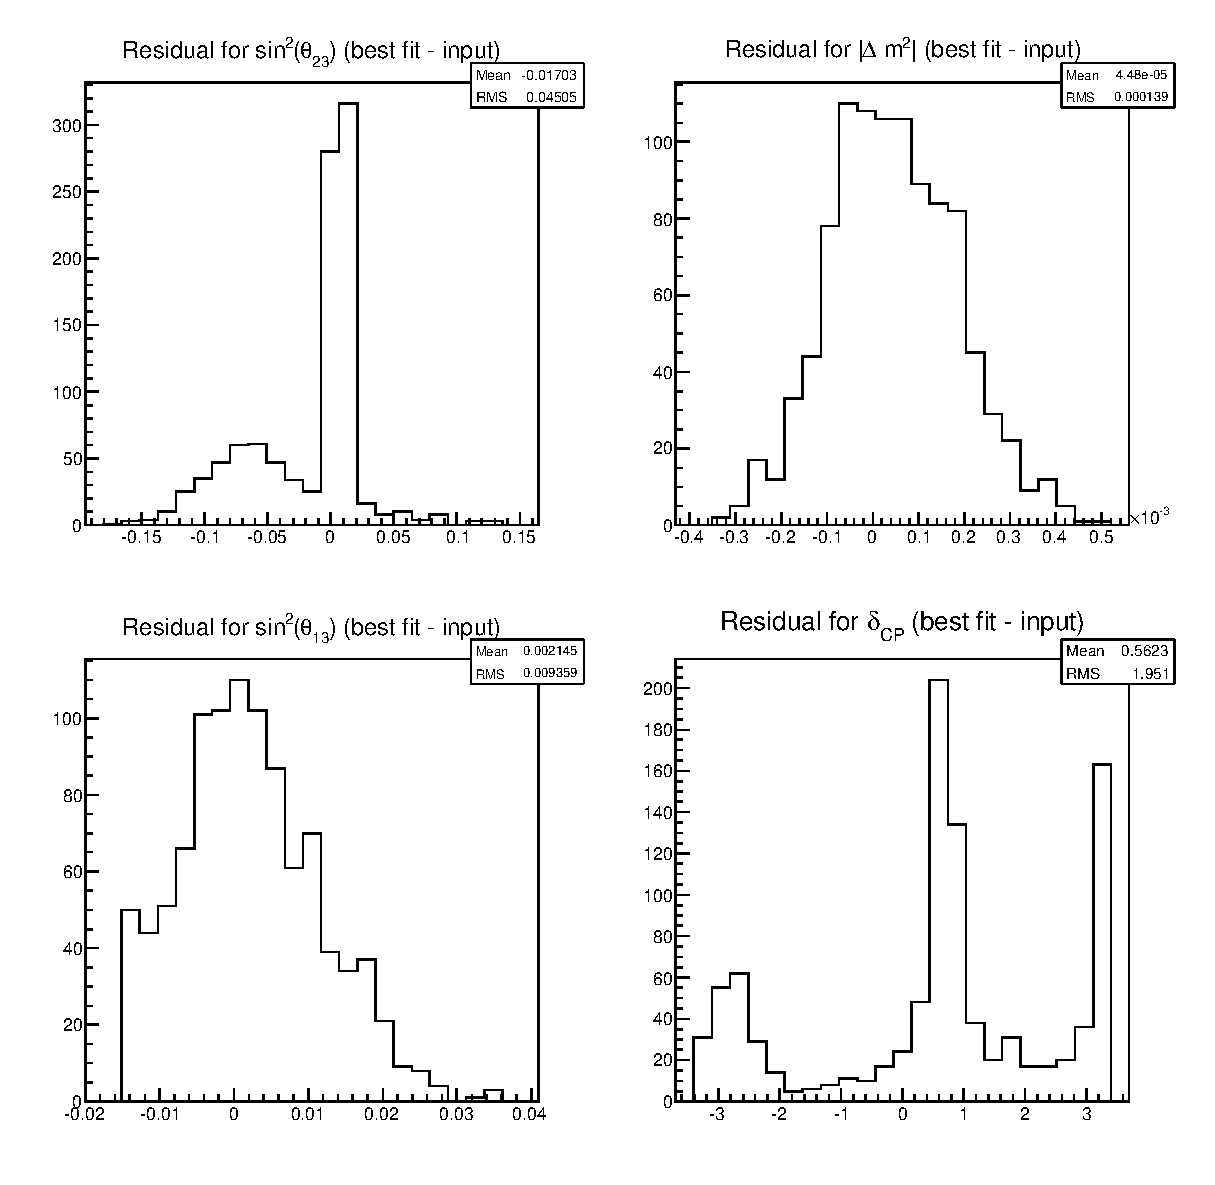
\includegraphics[width=18pc]{images/appendix/fitter_performance/Osc_residuals_nosyst_point3.eps}
\caption{
	Distribution of residuals of the four oscillation parameters in the '4 + 0' fit for oscillation point \# 3. 
 }
\label{fig:residuals_40_point3}
\end{minipage}
\hspace{0.02\linewidth}
\begin{minipage}[t]{0.5\linewidth}
\center
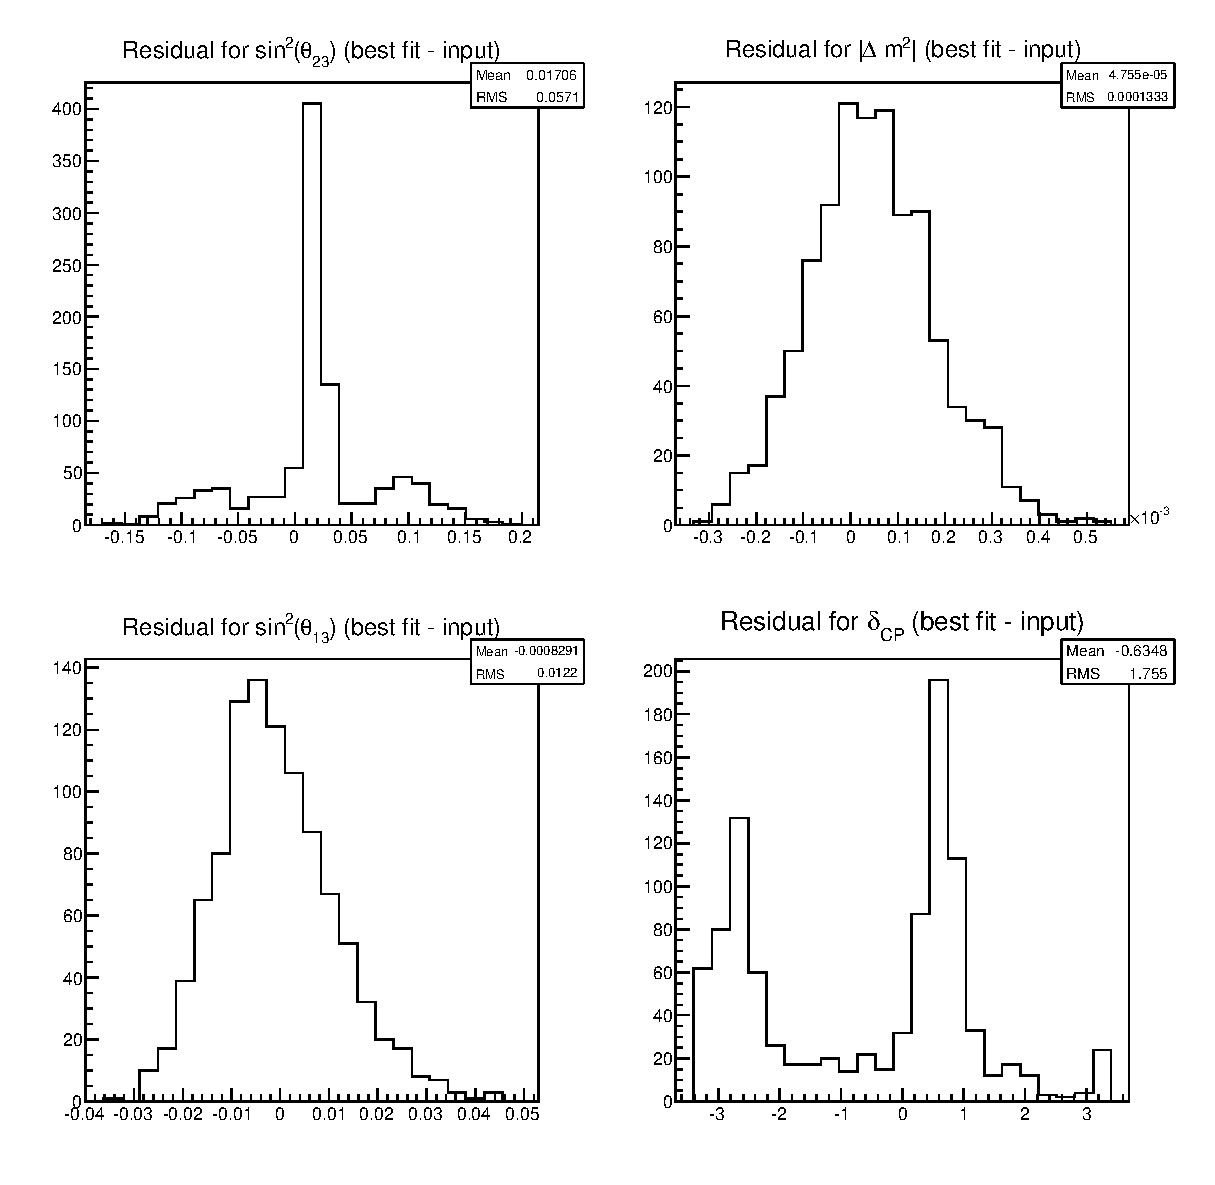
\includegraphics[width=18pc]{images/appendix/fitter_performance/Osc_residuals_nosyst_point4.eps}
\caption{
	Distribution of residuals of the four oscillation parameters in the '4 + 0' fit for oscillation point \# 4. 
 }
\end{minipage}

\end{figure*}


\begin{figure*}[htb]
\begin{minipage}[t]{0.5\linewidth}
\center
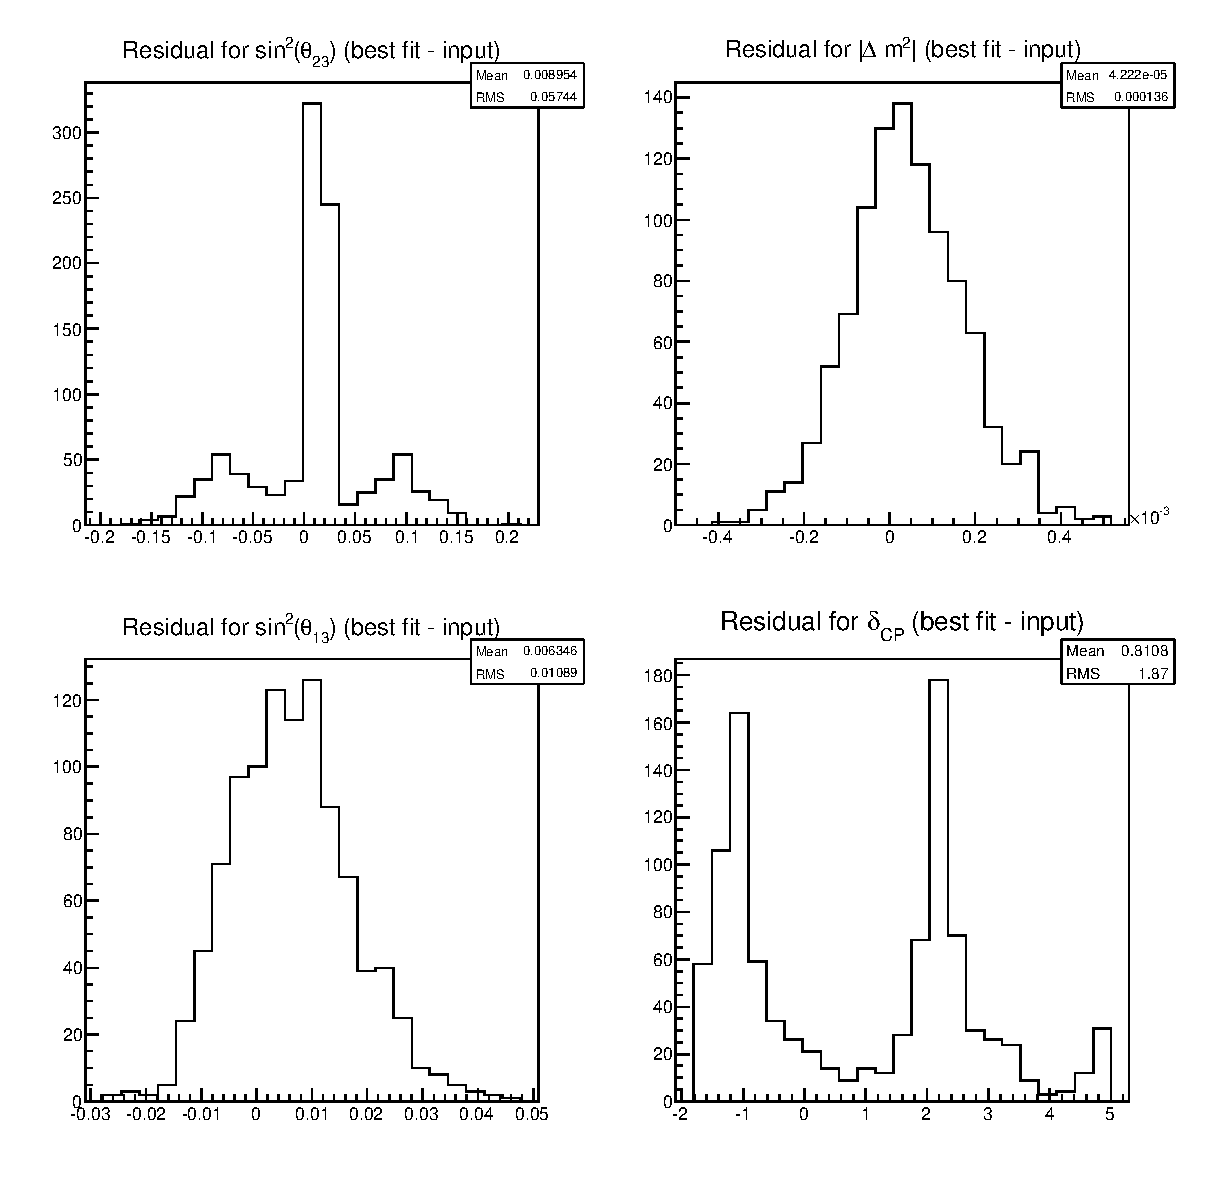
\includegraphics[width=18pc]{images/appendix/fitter_performance/Osc_residuals_nosyst_point5.eps}
\caption{
	Distribution of residuals of the four oscillation parameters in the '4 + 0' fit for oscillation point \# 5. 
 }
\label{fig:residuals_40_point5}
\end{minipage}
\hspace{0.02\linewidth}
\begin{minipage}[t]{0.5\linewidth}
\center
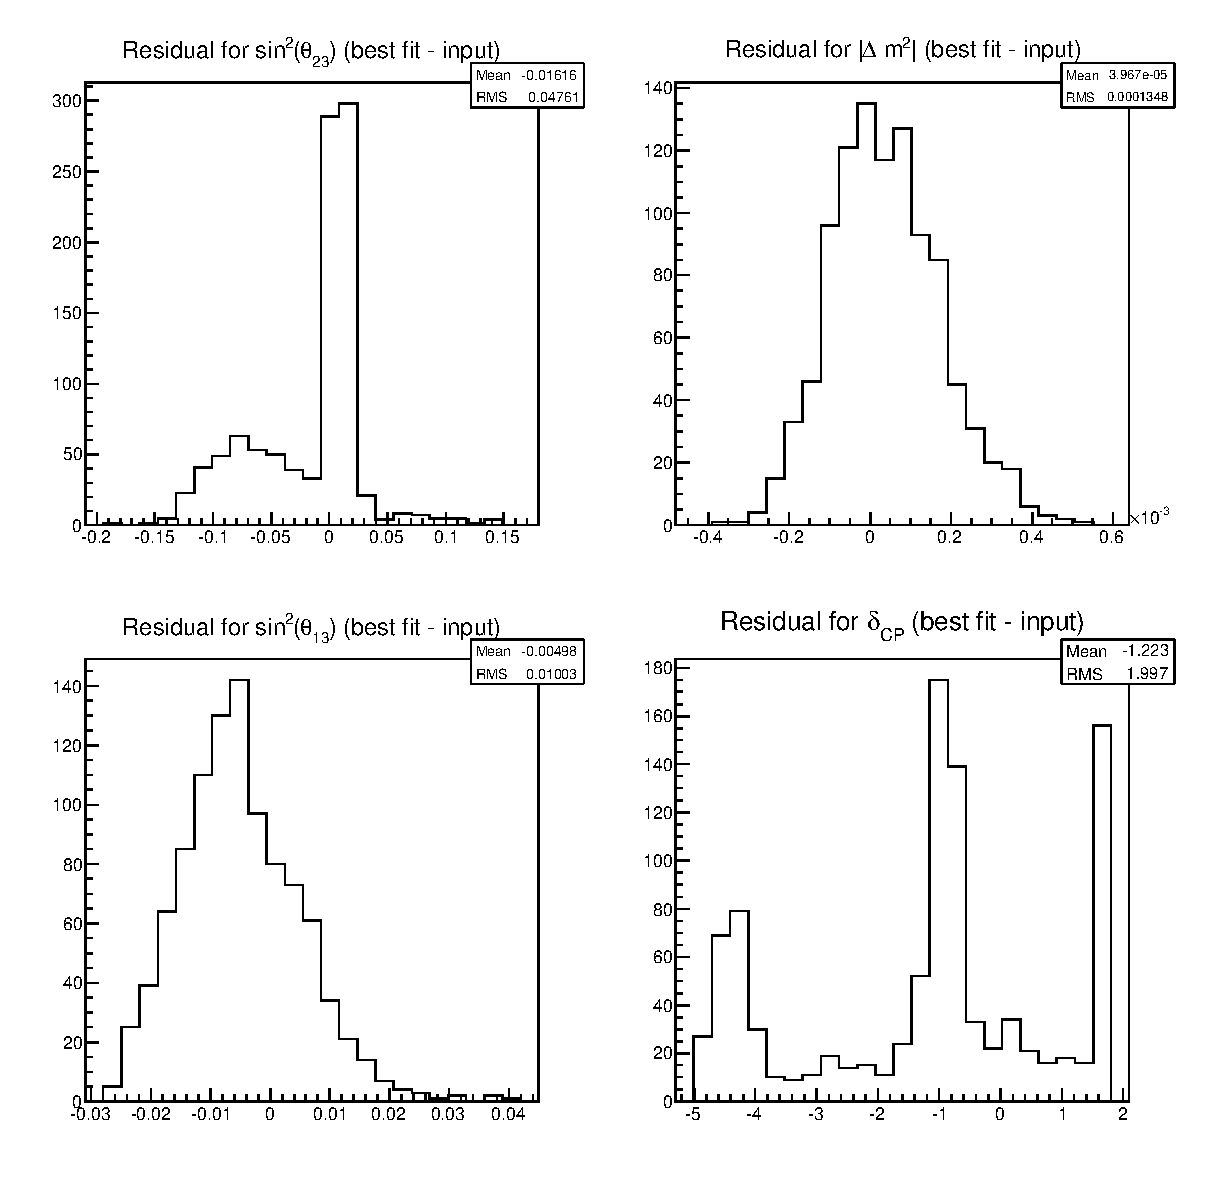
\includegraphics[width=18pc]{images/appendix/fitter_performance/Osc_residuals_nosyst_point6.eps}
\caption{
	Distribution of residuals of the four oscillation parameters in the '4 + 0' fit for oscillation point \# 6. 
 }
 \label{fig:residuals_40_point6}	
\end{minipage}

\end{figure*}

\clearpage

\begin{figure*}[htb]
\begin{minipage}[t]{0.5\linewidth}
\center
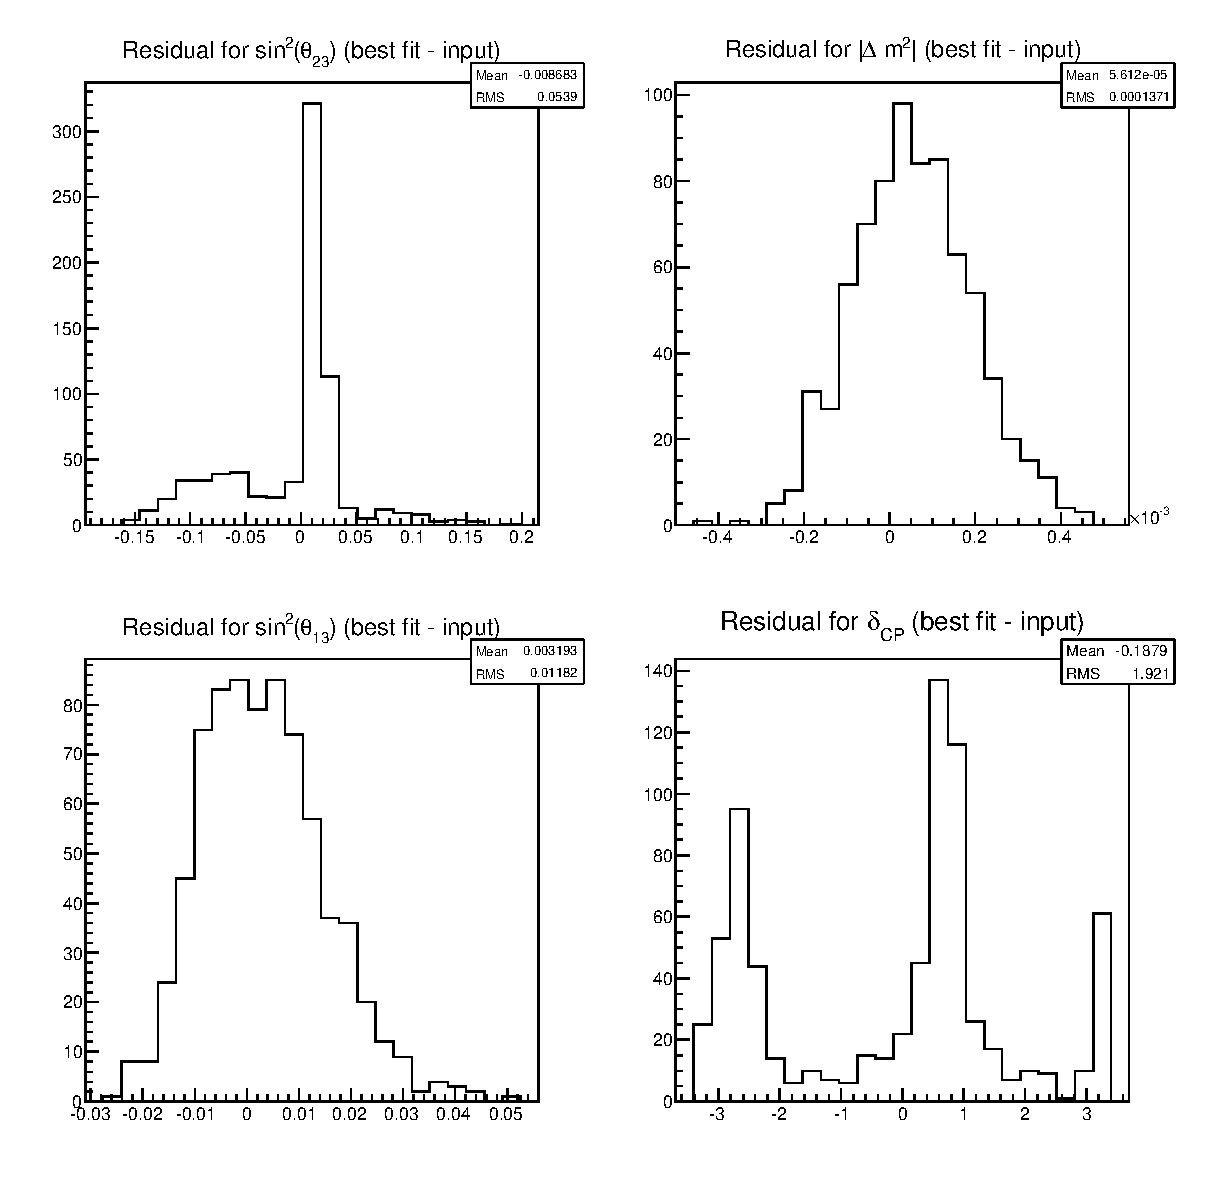
\includegraphics[width=18pc]{images/appendix/fitter_performance/Osc_residuals_nosyst_point7.eps}
\caption{
	Distribution of residuals of the four oscillation parameters in the '4 + 0' fit for oscillation point \# 7. 
 }
\label{fig:residuals_40_point7}
\end{minipage}
\hspace{0.02\linewidth}
\begin{minipage}[t]{0.5\linewidth}
\center
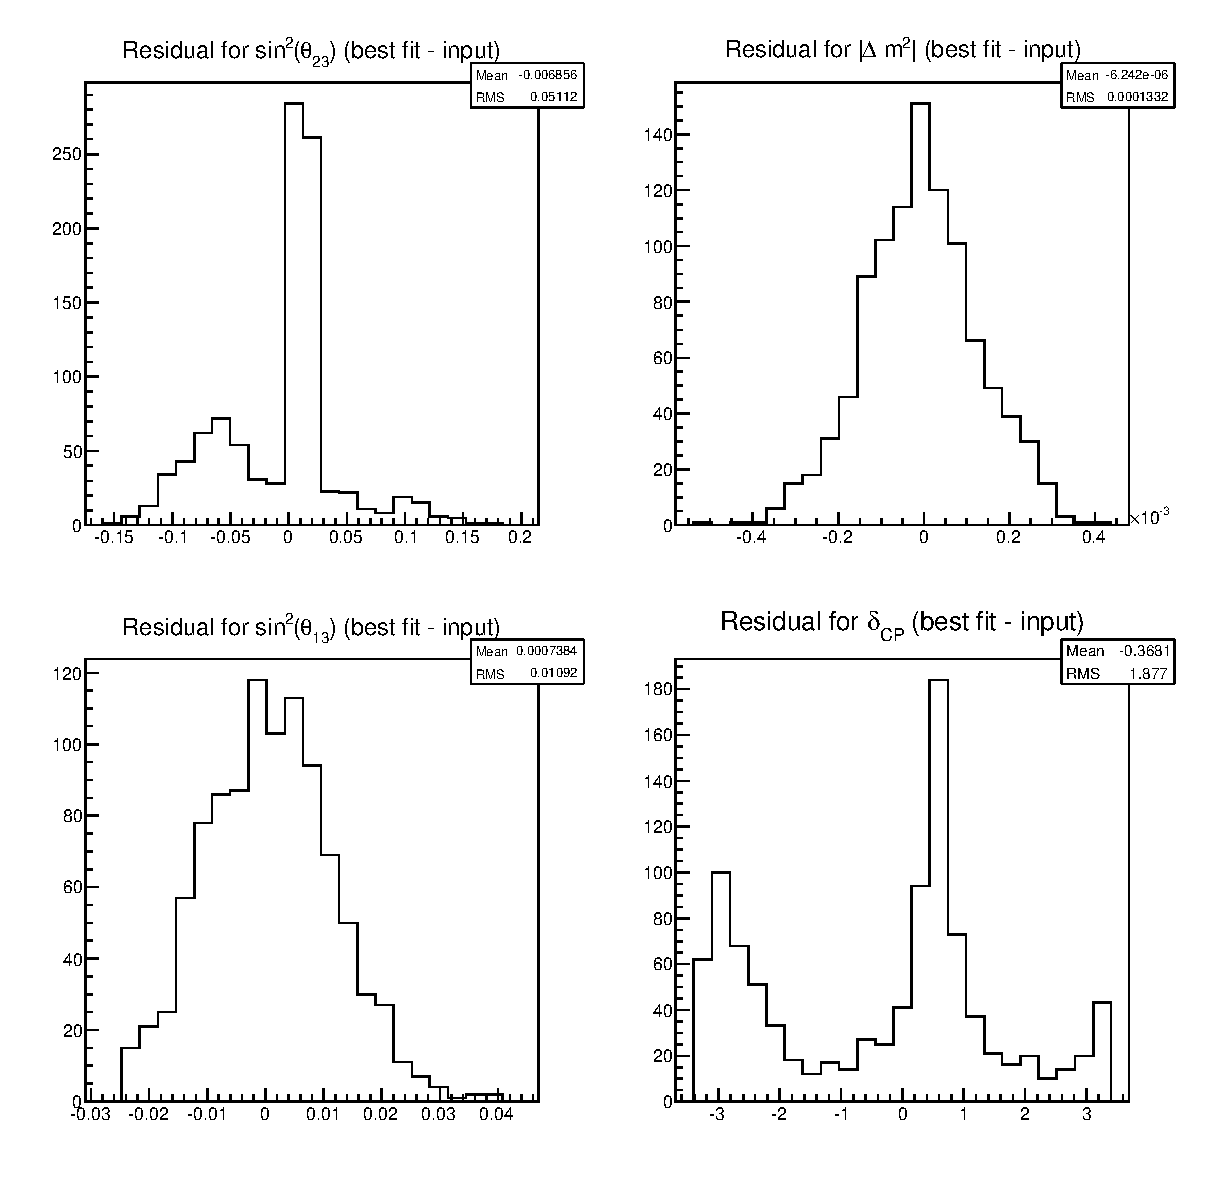
\includegraphics[width=18pc]{images/appendix/fitter_performance/Osc_residuals_nosyst_point8.eps}
\caption{
	Distribution of residuals of the four oscillation parameters in the '4 + 0' fit for oscillation point \# 8. 
 }
 \label{fig:residuals_40_last}
\end{minipage}

\end{figure*}





\begin{figure*}[htbc]
\center
%\begin{minipage}[t]{0.5\linewidth}
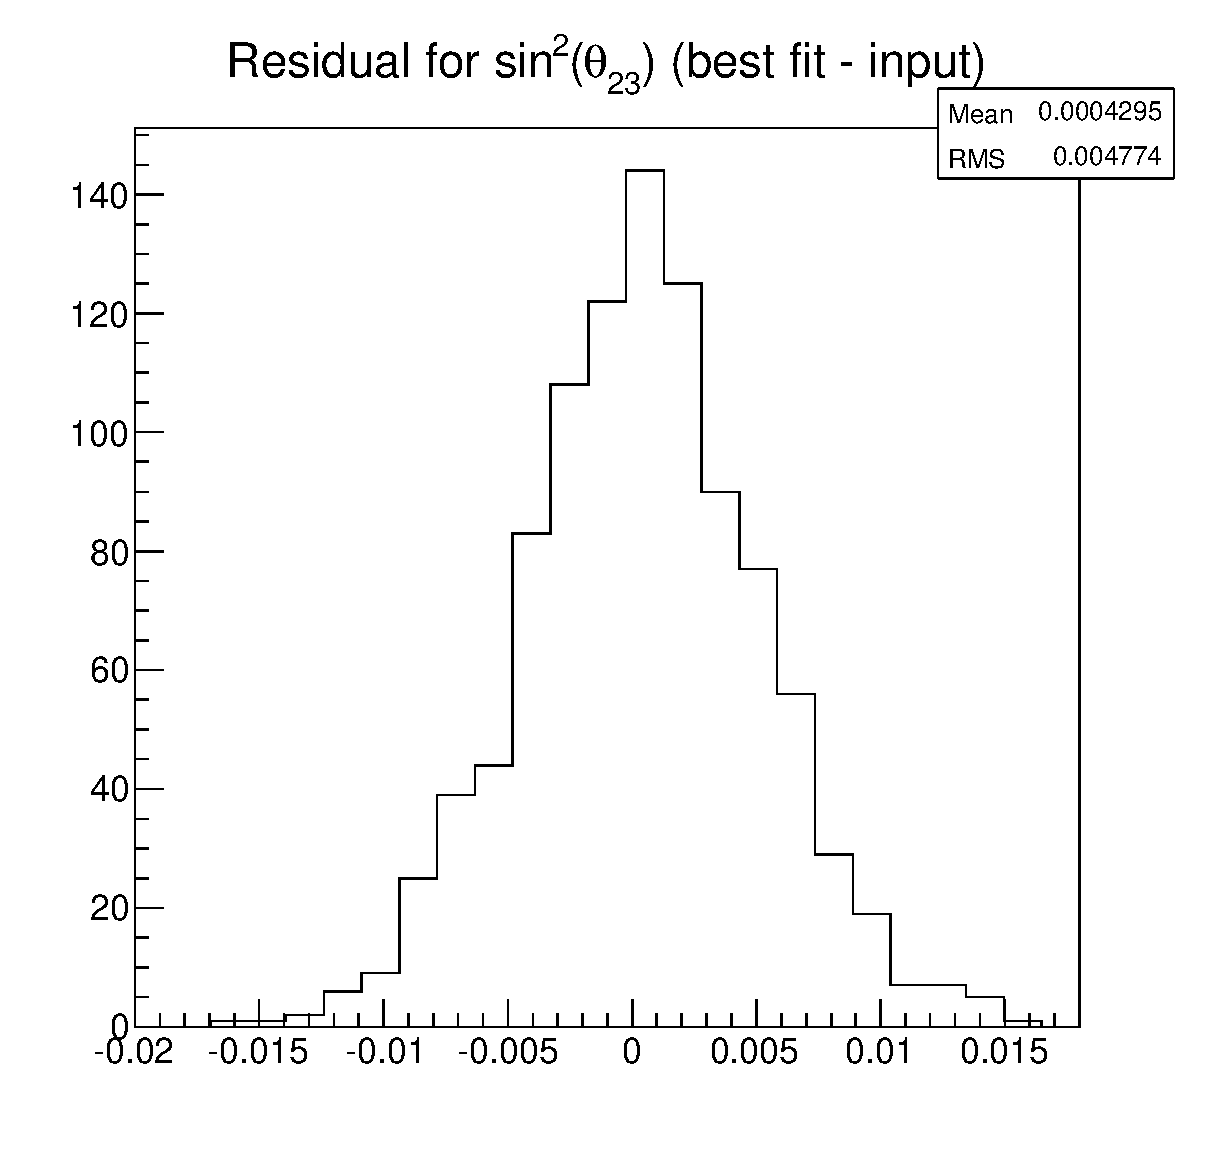
\includegraphics[width=18pc]{images/appendix/fitter_performance/Osc_residuals_nosyst_point1_x100.eps}
\caption{
	Distribution of residuals for $sin^{2}(\theta_{23})$ in the '4 + 0' fit for oscillation point \# 1 with $3.010 \times 10^{22}$ POT. 
 }
\label{fig:residuals_40_point1_x100}
%\end{minipage}
\end{figure*}



\clearpage

\subsection{'4 + 83' fit}

Figs.\ \ref{fig:residuals_483_first} - \ref{fig:residuals_483_last} show the distribution of residuals of the four oscillation parameters 
for each set described in table \ref{tab:osc_points} at $3.010 \times 10^{20}$ POT, with all systematic fluctuations.
As an example, Figs.\ \ref{fig:residuals_483_syst_first} - \ref{fig:residuals_483_syst_last} show the distribution of residuals for each systematic 
parameter for oscillation point \# 0. 
For the rest of oscillation points only summary plots showing the mean and its error ($\frac{RMS}{\sqrt{N}}$)  for all systematic parameters will be presented 
(Figs.\ \ref{fig:systematics_point0} - \ref{fig:systematics_point9})  
The numbering convention for the systematic parameters in those figures can  
be found in table \ref{tab:numbering_syst}. After comparing figures  \ref{fig:residuals_483_first} - \ref{fig:residuals_483_last} 
with  \ref{fig:residuals_40_first} - \ref{fig:residuals_40_last} it can be concluded that fitting all systematics does not change 
the distributions of residuals for the oscillation parameters.
From Figs.\ \ref{fig:systematics_point0} - \ref{fig:systematics_point9} there are three systematics with a "biased" mean of 
the distribution of residuals. The reason for this was found and will be explained now. 
Apart from that there are still no unexpected features.

The three systematics with a "biased" mean of the distribution of residuals are:

\begin{enumerate}
\item{{\bf Spectral function}: The reason for the distribution of residuals for this parameter to be "biased" is the special distribution function used to tweak this systematic parameter, which is uniform from 0 to 1, centered at 0.5, instead of gaussian.		
It was checked that when using a gaussian distribution as for the rest, this "bias" disappeared. However, the use of a uniform function will be kept for this parameter as it was done for the disappearance analysis.
}
\item{{\bf Pi-less delta decay}:The explanation for the "bias" in its distribution of residuals comes from the special response function used for this for this parameter, 
which was only calculated up to $-1\sigma$ and then propagated to $-3\sigma$ with the same value as for $-1\sigma$.
This pathology disappears when constraining this parameter with boundaries $-1\sigma$ to $1\sigma$. 
}
\item{{\bf $1R_{\mu}$ NC efficiency}:The reason for this parameter to have a "biased" distribution of residuals comes from the low statistics at current POT.
When Poisson fluctuations are made of the bin contents of the $E_{reco}$ distributions, a downward fluctuation is more likely than an upward fluctuation (see replies to comments and revision history for TN141).
Adding the fact that the NC modes are distributed around the oscillation maximum, the (most likely) downwards Poisson fluctuations translate into a (most likely) negative value of the NC efficiency, explaining a "bias" to negative values for this parameter.
It was checked that the "bias" in the distribution depends on the true input value of $sin^{2}\theta_{23}$, disappearing when $sin^{2}\theta_{23}$ is far away from 0.5; and also that it decreases as well when increasing the POT. 
}
\end{enumerate}


\begin{table}[htbp]
\center
\begin{tabular}{|p{3cm}|p{7cm}|}
\hline 
\# & Systematic \\
\hline 
0 -24 & BANFF $\nu_{\mu}$, $\bar{\nu_{\mu}}$, $\nu_{e}$ and $\bar{\nu_{e}}$ flux bins \\
25  & BANFF CCQE axial mass \\
26 & BANFF resonance-production axial mass \\
27-29 & CCQE normalization \\
30-31 & CC 1$\pi$ normalization \\
32 & NC1$\pi0$ \\
\hline
33 & Fermi momentum \\
34 & Nuclear modeling (Spectral function) \\
35 & Binding energy \\
36 & Shape of $\pi$ momentum distribution (W shape) \\
37 & CC other shape\\
38 & $\pi$-less $\Delta$ decay\\
39 & CC coherent normalization \\
40 & NC 1$\pi^{\pm}$ normalization \\
41 & NC coherent normalization \\
42 & NC other normalizarion \\
43 & $\sigma_{\nu_{e}}/\sigma_{\nu_{\mu}}$ ratio \\
44 & $\sigma_{\bar{\nu}}/\sigma_{\nu}$ ratio \\
\hline
45 & Reconstructed energy scale \\
46-48 & $\nu_{\mu}$, $\bar{\nu_{\mu}}$ CCQE ring counting efficiency \\
49 & $\nu_{\mu}$, $\bar{\nu_{\mu}}$ CCQE other efficiency \\
50 & $\nu_{\mu}$, $\bar{\nu_{\mu}}$ CCnonQE efficiency \\
51 & NC efficiency \\
52 & $\nu_{e}$, $\bar{\nu_{e}}$ CC efficiency \\
53-55 & 1$R_{e}$ osc. $\nu_{e}$ CC efficiency \\
56-58 & 1$R_{e}$ $\nu_{\mu}$, $\bar{\nu_{\mu}}$ CC efficiency \\
59-61 & 1$R_{e}$ $\nu_{e}$, $\bar{\nu_{e}}$ CC efficiency \\
62-64 & 1$R_{e}$ NC efficiency \\
\hline
65-67 & 1$R_{\mu}$  FSI: $\nu_{\mu}$, $\bar{\nu_{\mu}}$ CCQE  \\
68 & $R_{\mu}$  FSI: $\nu_{\mu}$, $\bar{\nu_{\mu}}$ CCnonQE efficiency \\
69 & $R_{\mu}$  FSI: $\nu_{e}$, $\bar{\nu_{e}}$ CC\\
70 & $R_{\mu}$  FSI: NC  \\
\hline
71-73 & 1$R_{e}$ FS: osc. $\nu_{e}$ CC  \\
74-76 & 1$R_{e}$ FSI: $\nu_{\mu}$, $\bar{\nu_{\mu}}$ CC  \\
77-79 & 1$R_{e}$ FSI: $\nu_{e}$, $\bar{\nu_{e}}$ CC  \\
80-82 & 1$R_{e}$ FSI: NC  \\
\hline
\end{tabular}\\[2pt]
\caption{
  The numbering of systematic parameters for figures  \ref{fig:systematics_point0} - \ref{fig:systematics_point9} 
}
\label{tab:numbering_syst}
\end{table}



\clearpage



\begin{figure*}[htb]
\begin{minipage}[t]{0.5\linewidth}
\center
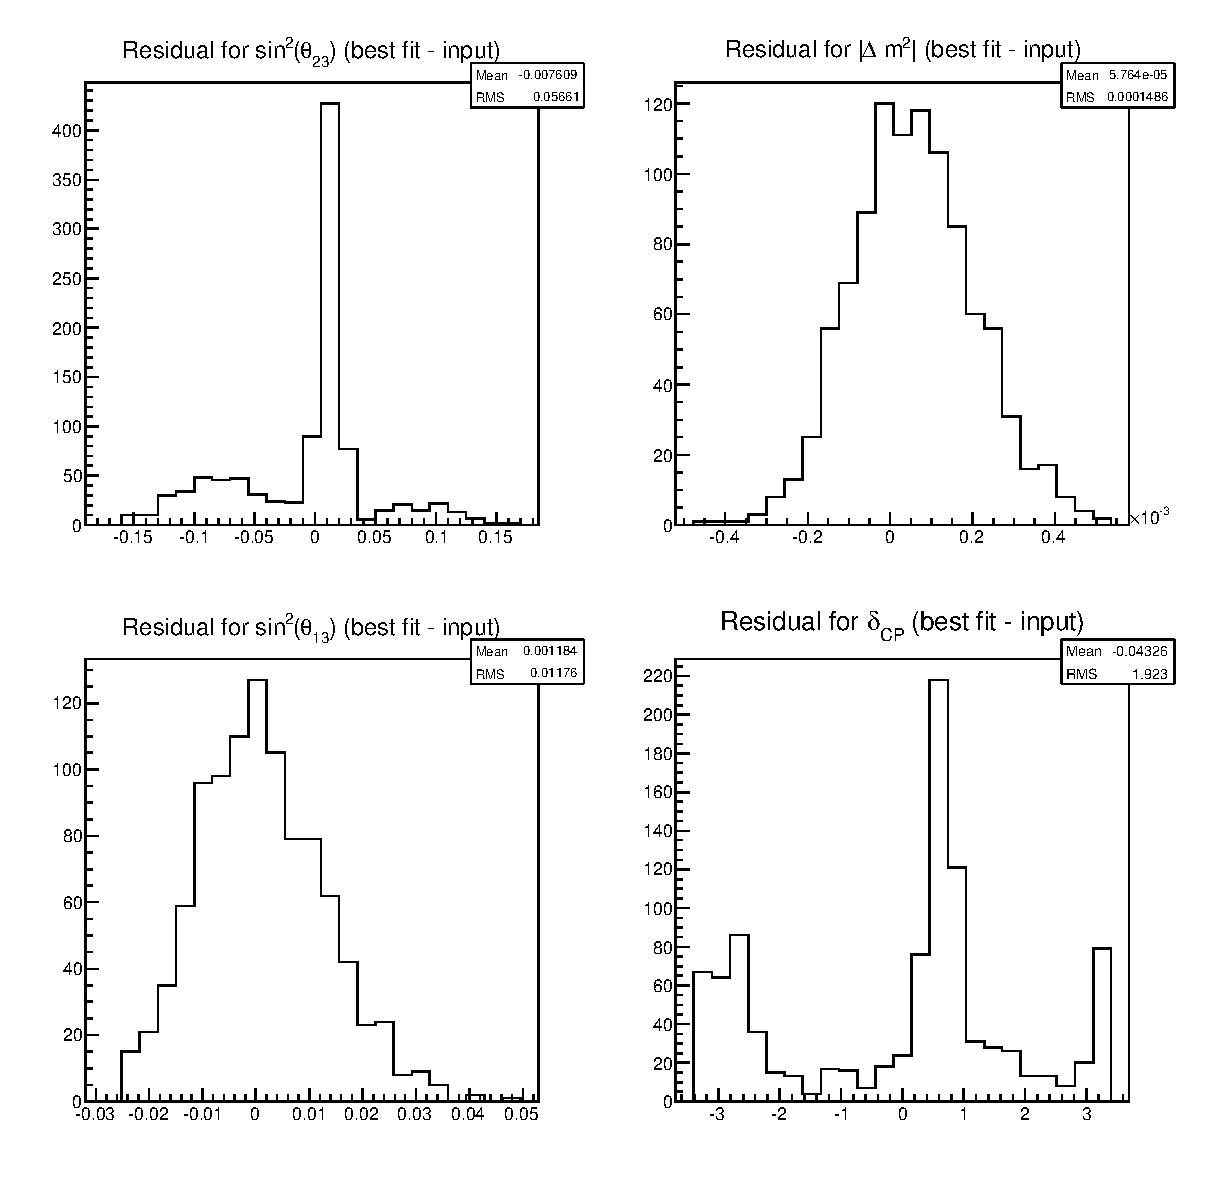
\includegraphics[width=18pc]{images/appendix/fitter_performance/Osc_residuals_joint_syst_point0.eps}
\caption{
	Distribution of residuals of the four oscillation parameters in the '4 + 83' fit for oscillation point \# 0. 
 }
\label{fig:residuals_483_first}
\end{minipage}
\hspace{0.02\linewidth}
\begin{minipage}[t]{0.5\linewidth}
\center
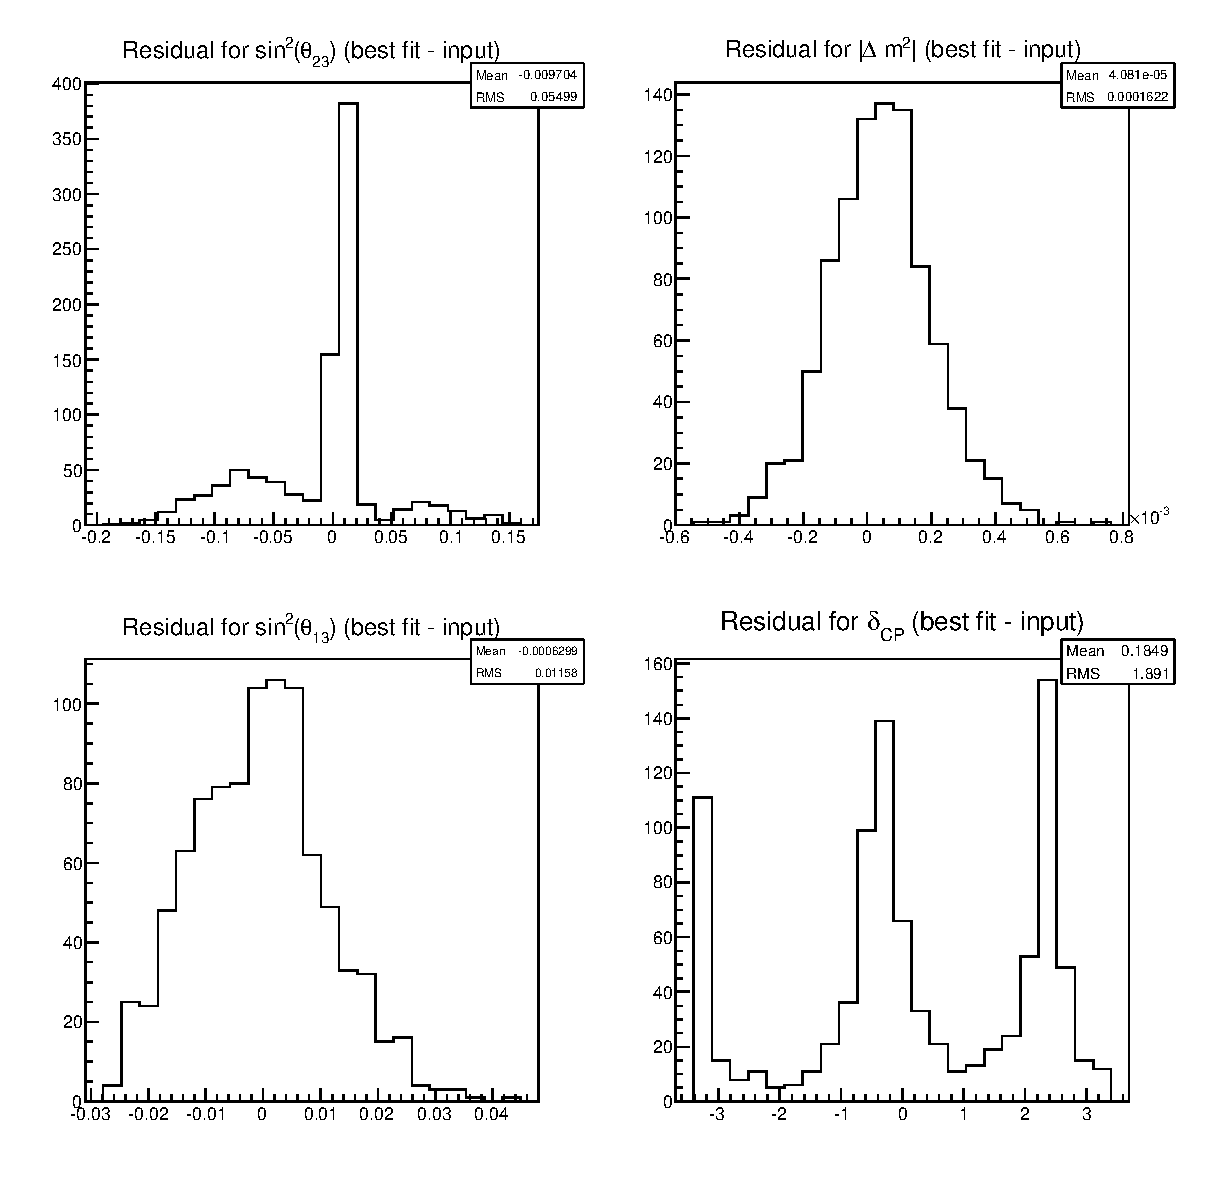
\includegraphics[width=18pc]{images/appendix/fitter_performance/Osc_residuals_joint_syst_point9.eps}
\caption{
	Distribution of residuals of the four oscillation parameters in the '4 + 83' fit for oscillation point \# 9. 
 }
\end{minipage}

\end{figure*}


\begin{figure*}[htb]
\begin{minipage}[t]{0.5\linewidth}
\center
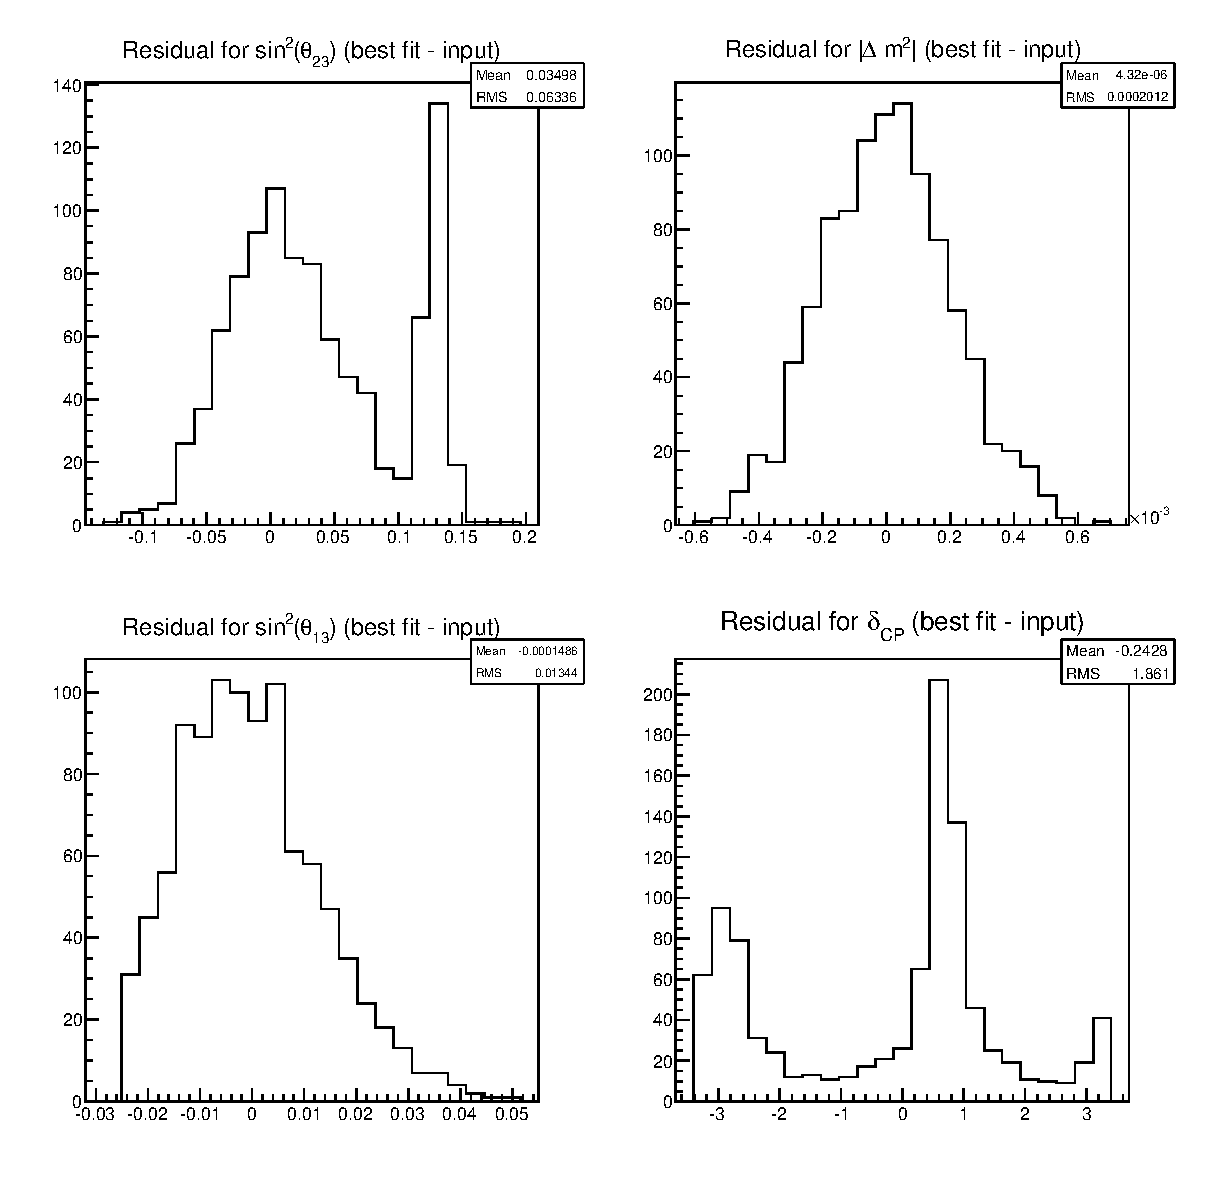
\includegraphics[width=18pc]{images/appendix/fitter_performance/Osc_residuals_joint_syst_point1.eps}
\caption{
	Distribution of residuals of the four oscillation parameters in the '4 + 83' fit for oscillation point \# 1. 
 }
\label{fig:residuals_483_point1}
\end{minipage}
\hspace{0.02\linewidth}
\begin{minipage}[t]{0.5\linewidth}
\center
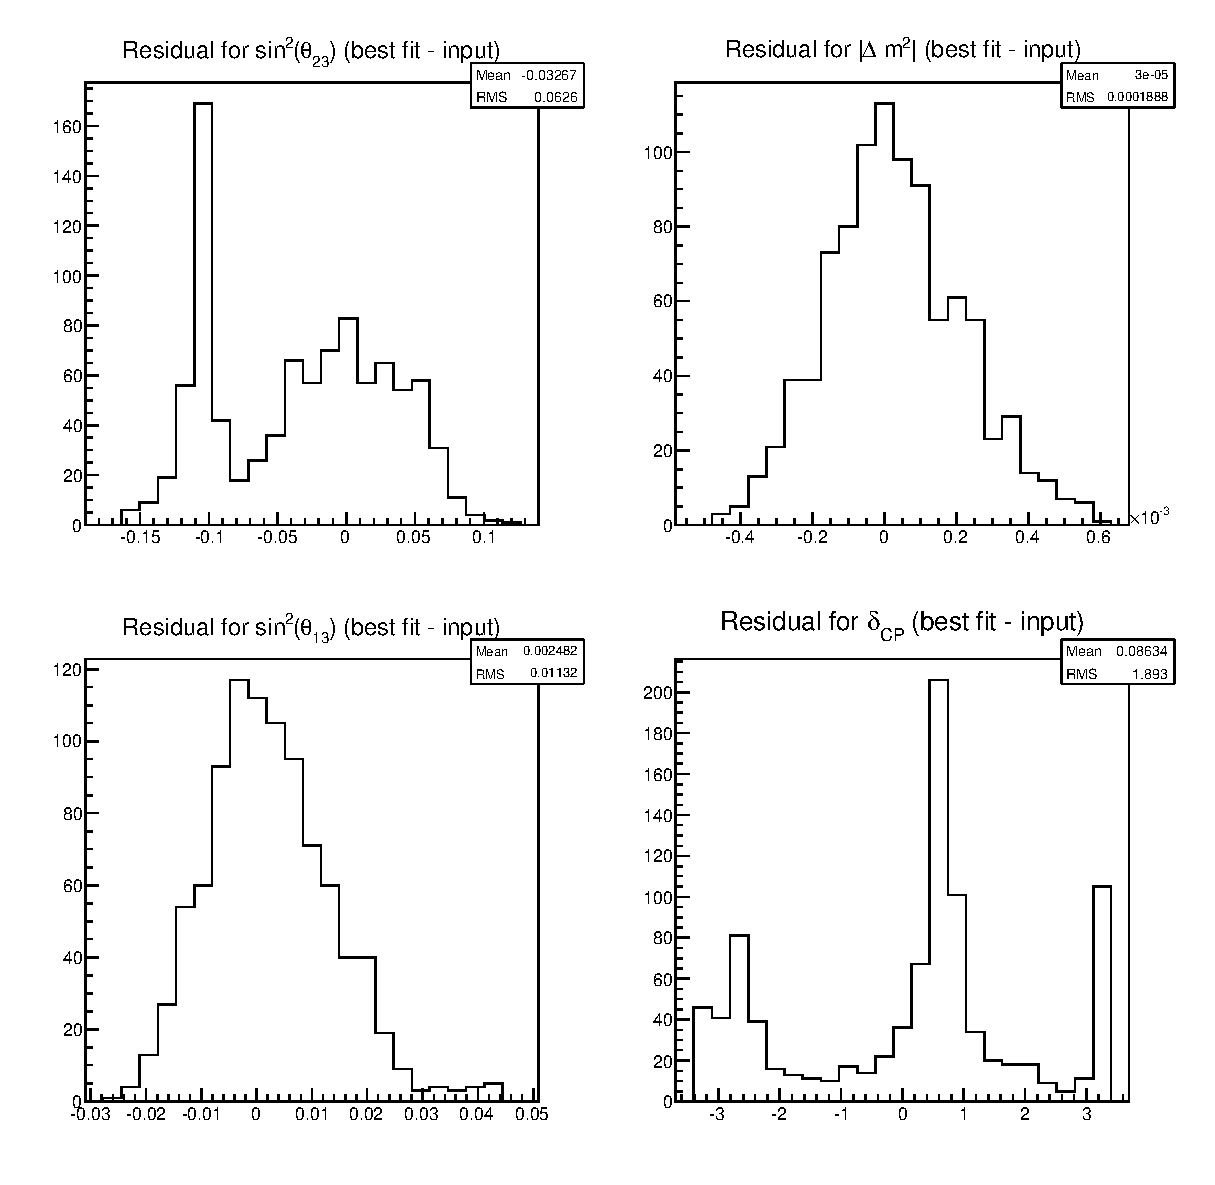
\includegraphics[width=18pc]{images/appendix/fitter_performance/Osc_residuals_joint_syst_point2.eps}
\caption{
	Distribution of residuals of the four oscillation parameters in the '4 + 83' fit for oscillation point \# 2. 
 }
\end{minipage}

\end{figure*}

\clearpage

\begin{figure*}[htb]
\begin{minipage}[t]{0.5\linewidth}
\center
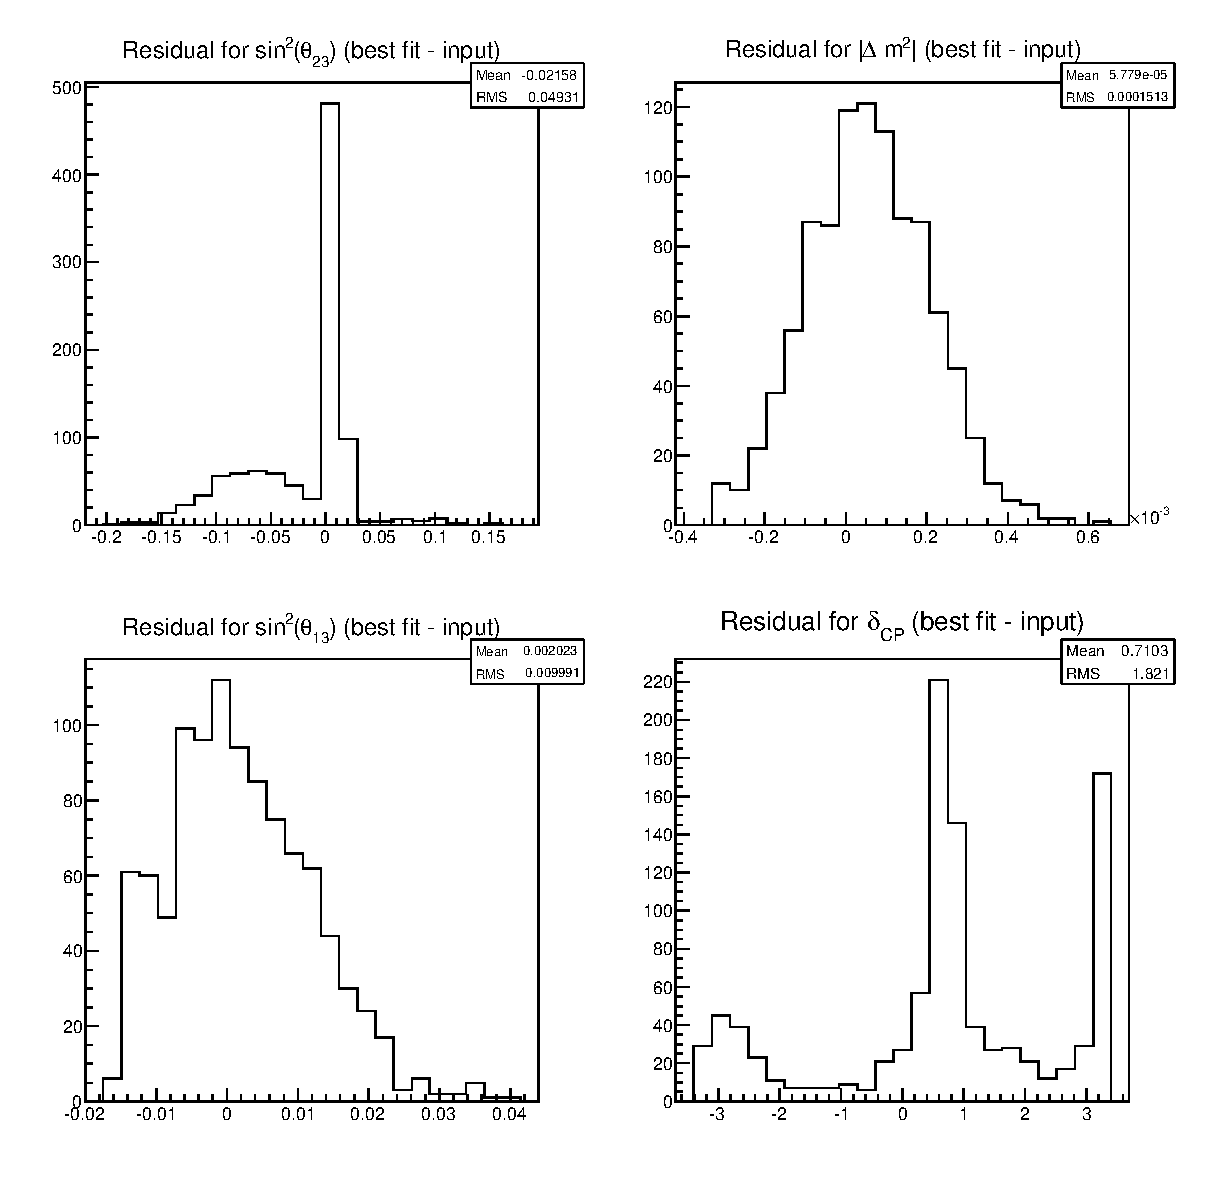
\includegraphics[width=18pc]{images/appendix/fitter_performance/Osc_residuals_joint_syst_point3.eps}
\caption{
	Distribution of residuals of the four oscillation parameters in the '4 + 83' fit for oscillation point \# 3. 
 }
\label{fig:residuals_483_point3}
\end{minipage}
\hspace{0.02\linewidth}
\begin{minipage}[t]{0.5\linewidth}
\center
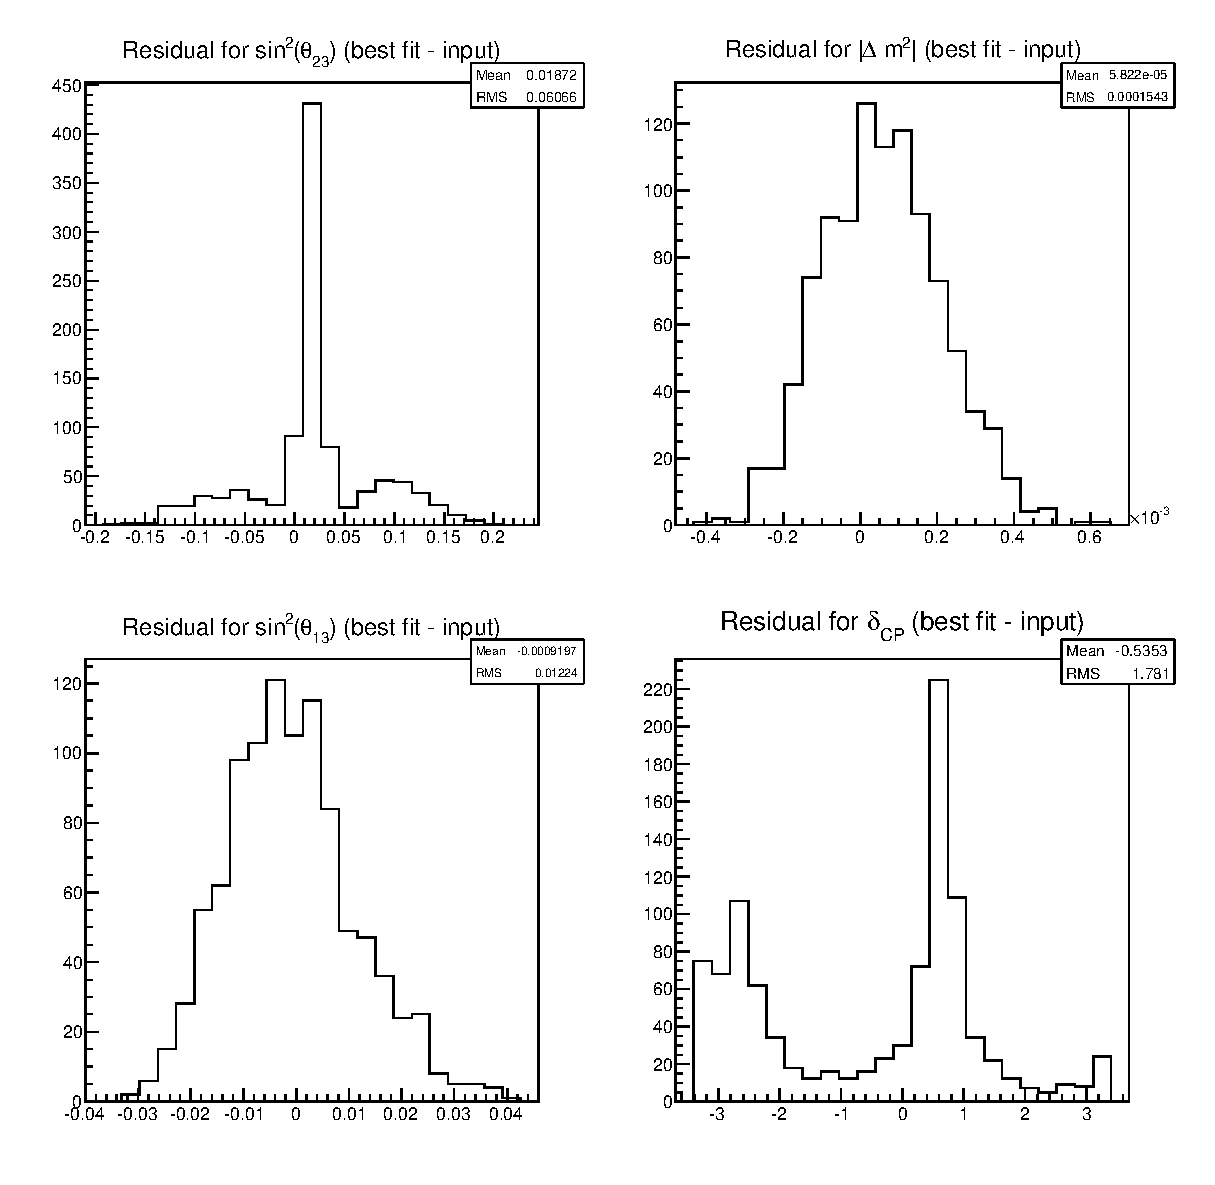
\includegraphics[width=18pc]{images/appendix/fitter_performance/Osc_residuals_joint_syst_point4.eps}
\caption{
	Distribution of residuals of the four oscillation parameters in the '4 + 83' fit for oscillation point \# 4. 
 }
\end{minipage}

\end{figure*}


\begin{figure*}[htb]
\begin{minipage}[t]{0.5\linewidth}
\center
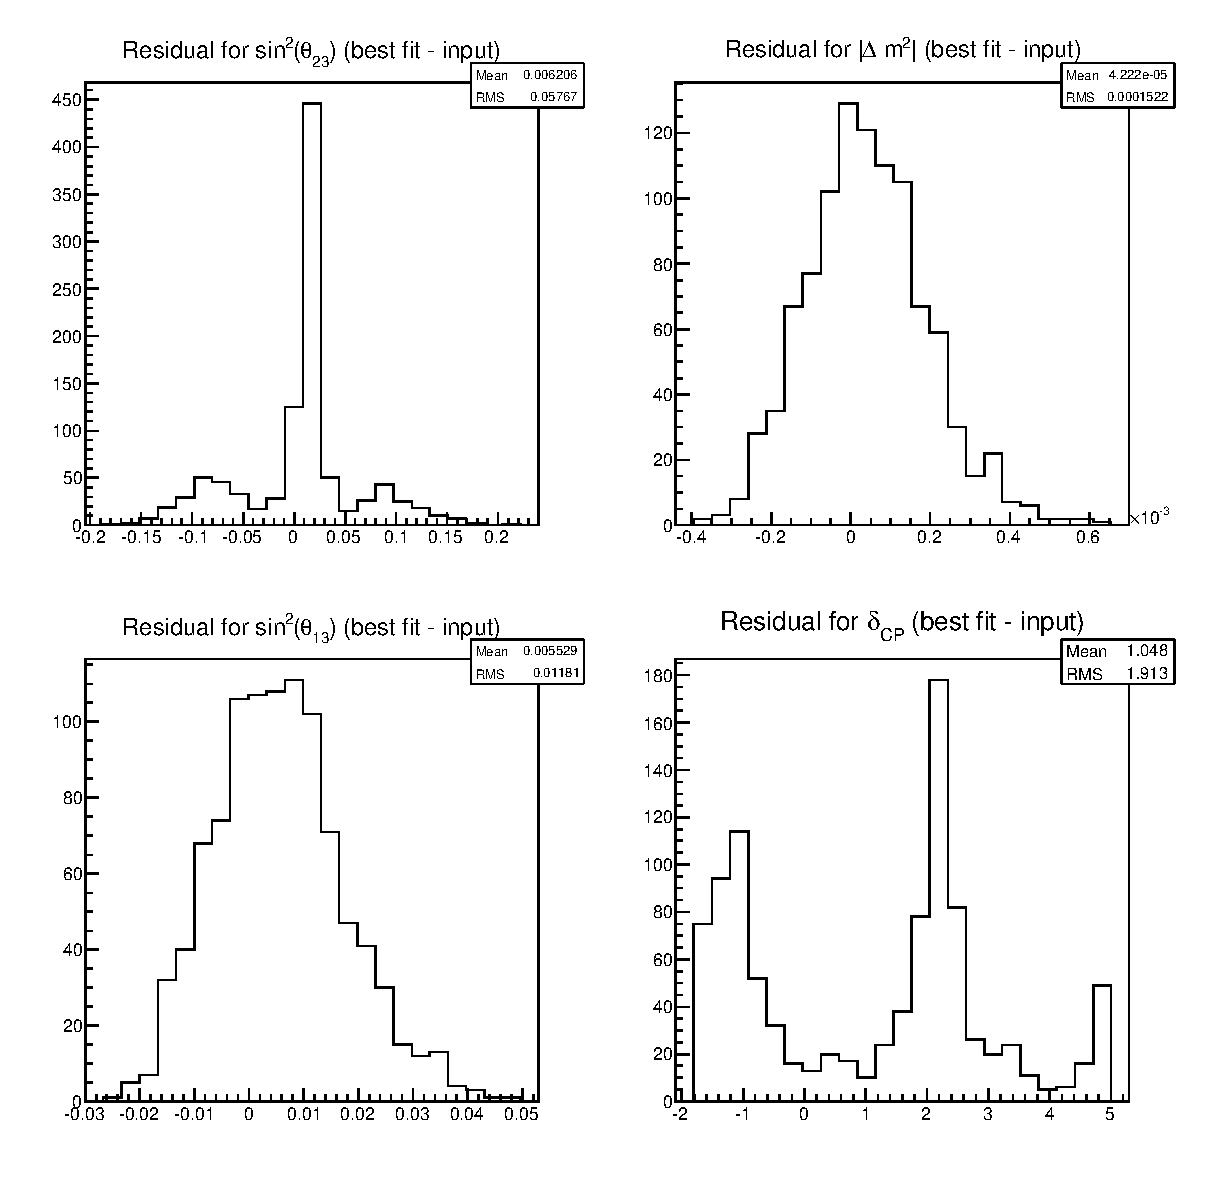
\includegraphics[width=18pc]{images/appendix/fitter_performance/Osc_residuals_joint_syst_point5.eps}
\caption{
	Distribution of residuals of the four oscillation parameters in the '4 + 83' fit for oscillation point \# 5. 
 }
\label{fig:residuals_483_point5}
\end{minipage}
\hspace{0.02\linewidth}
\begin{minipage}[t]{0.5\linewidth}
\center
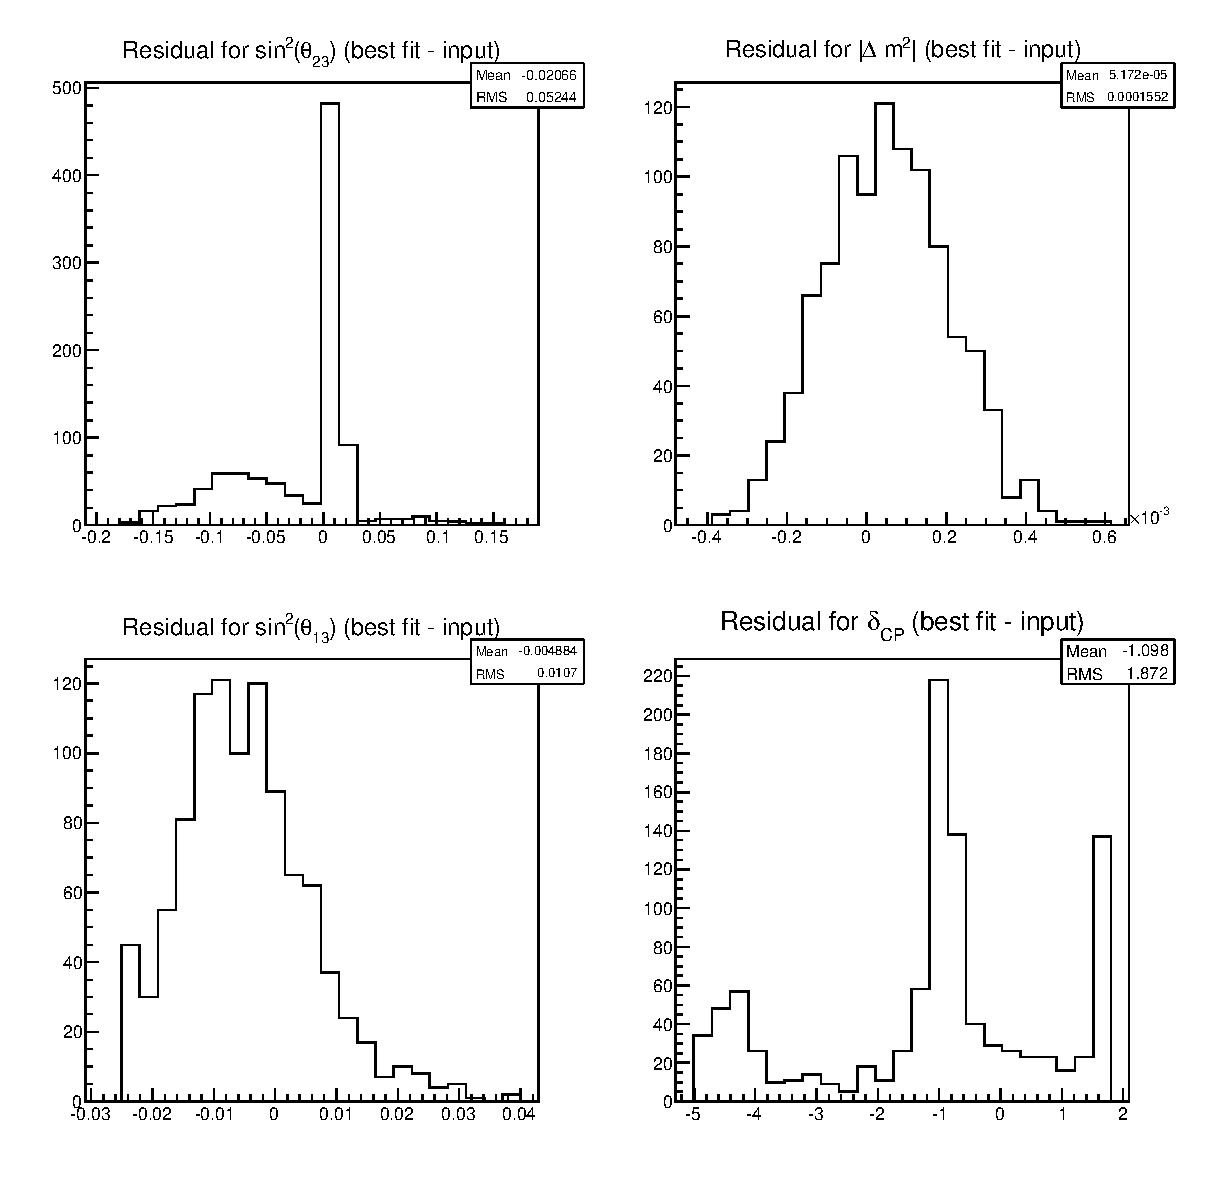
\includegraphics[width=18pc]{images/appendix/fitter_performance/Osc_residuals_joint_syst_point6.eps}
\caption{
	Distribution of residuals of the four oscillation parameters in the '4 + 83' fit for oscillation point \# 6. 
 }
\end{minipage}

\end{figure*}

\clearpage

\begin{figure*}[htb]
\begin{minipage}[t]{0.5\linewidth}
\center
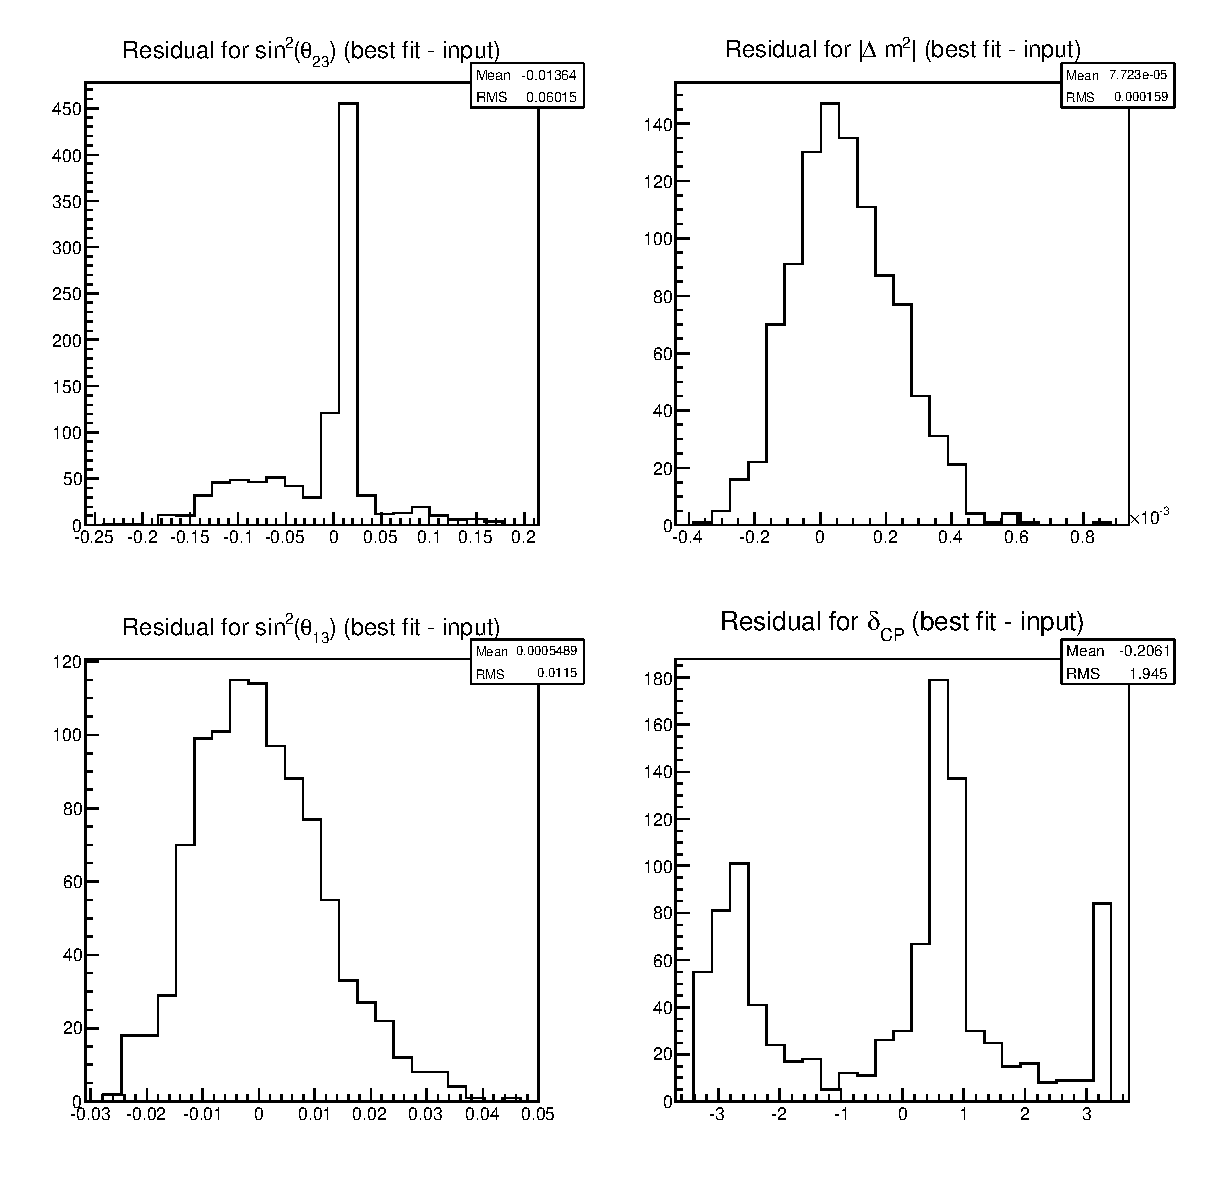
\includegraphics[width=18pc]{images/appendix/fitter_performance/Osc_residuals_joint_syst_point7.eps}
\caption{
	Distribution of residuals of the four oscillation parameters in the '4 + 83' fit for oscillation point \# 7. 
 }
\label{fig:residuals_483_point7}
\end{minipage}
\hspace{0.02\linewidth}
\begin{minipage}[t]{0.5\linewidth}
\center
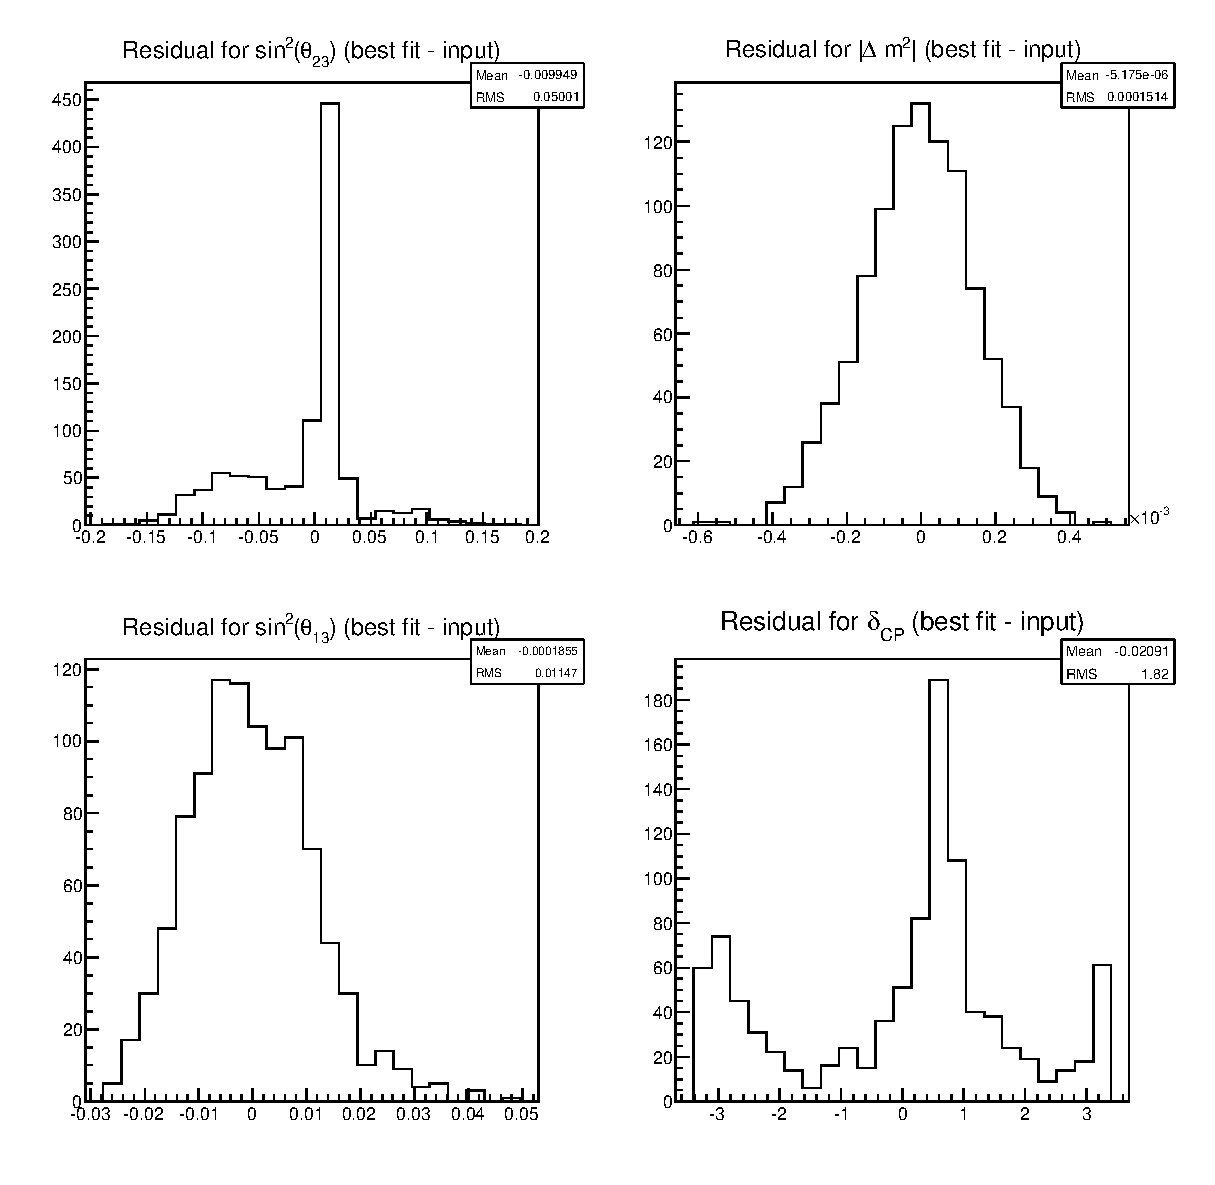
\includegraphics[width=18pc]{images/appendix/fitter_performance/Osc_residuals_joint_syst_point8.eps}
\caption{
	Distribution of residuals of the four oscillation parameters in the '4 + 83' fit for oscillation point \# 8. 
 }
 \label{fig:residuals_483_last}
\end{minipage}

\end{figure*}

\clearpage

%%%% SYSTEMATICS %%%

\begin{figure*}[htbc]	
\center
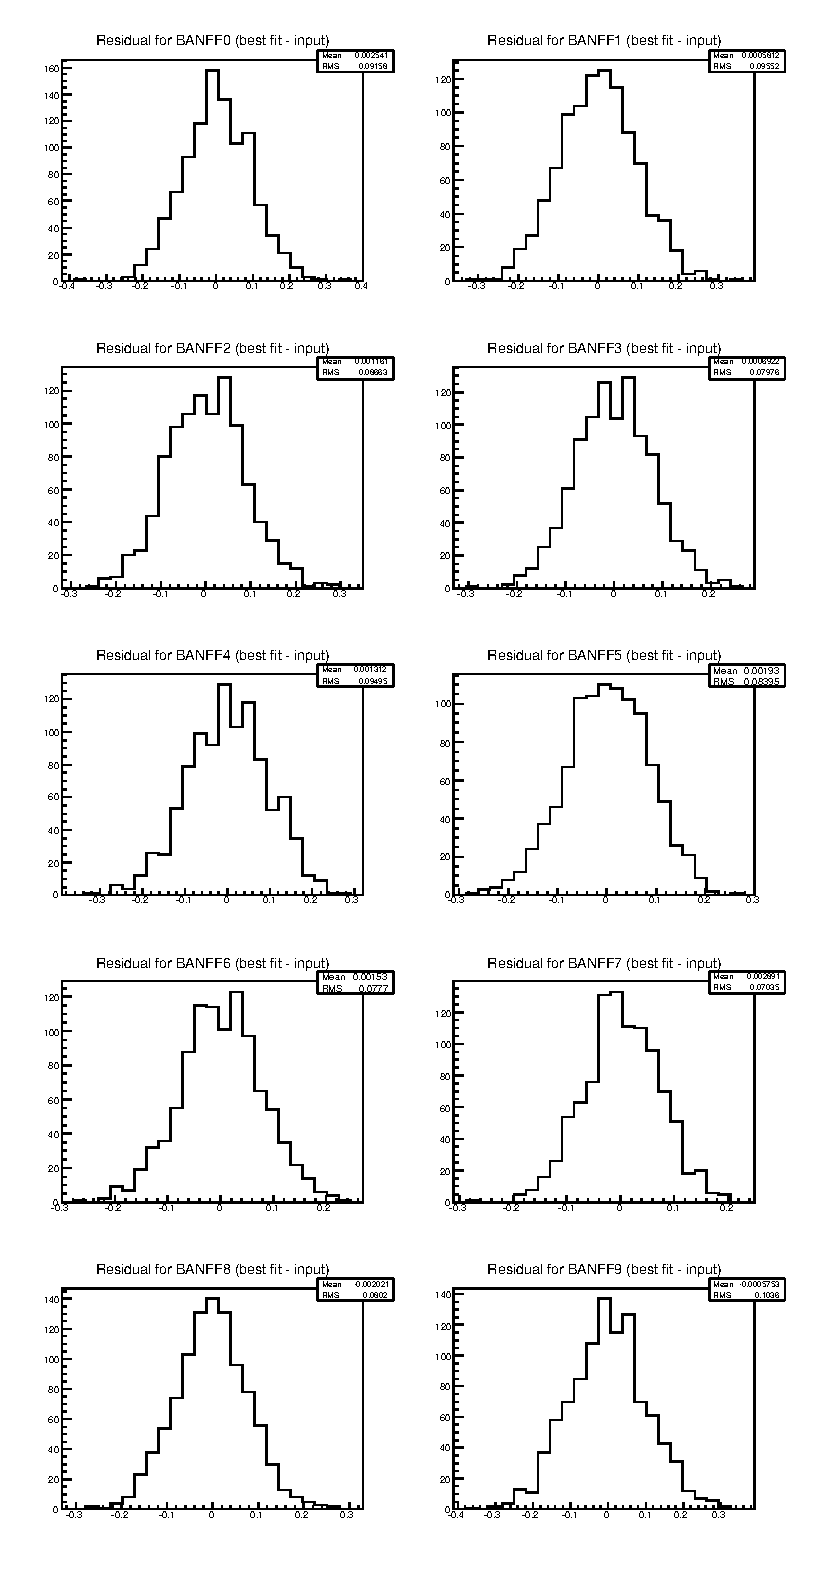
\includegraphics[width=25pc]{images/appendix/fitter_performance/Syst1_residuals_joint_syst_point0.eps}
\caption{
	Distribution of residuals of the BANFF (0-9) systematic parameters in the '4 + 83' fit for oscillation point \# 0. 
 }
\label{fig:residuals_483_syst_first}
\end{figure*}


\begin{figure*}[htbc]	
\center
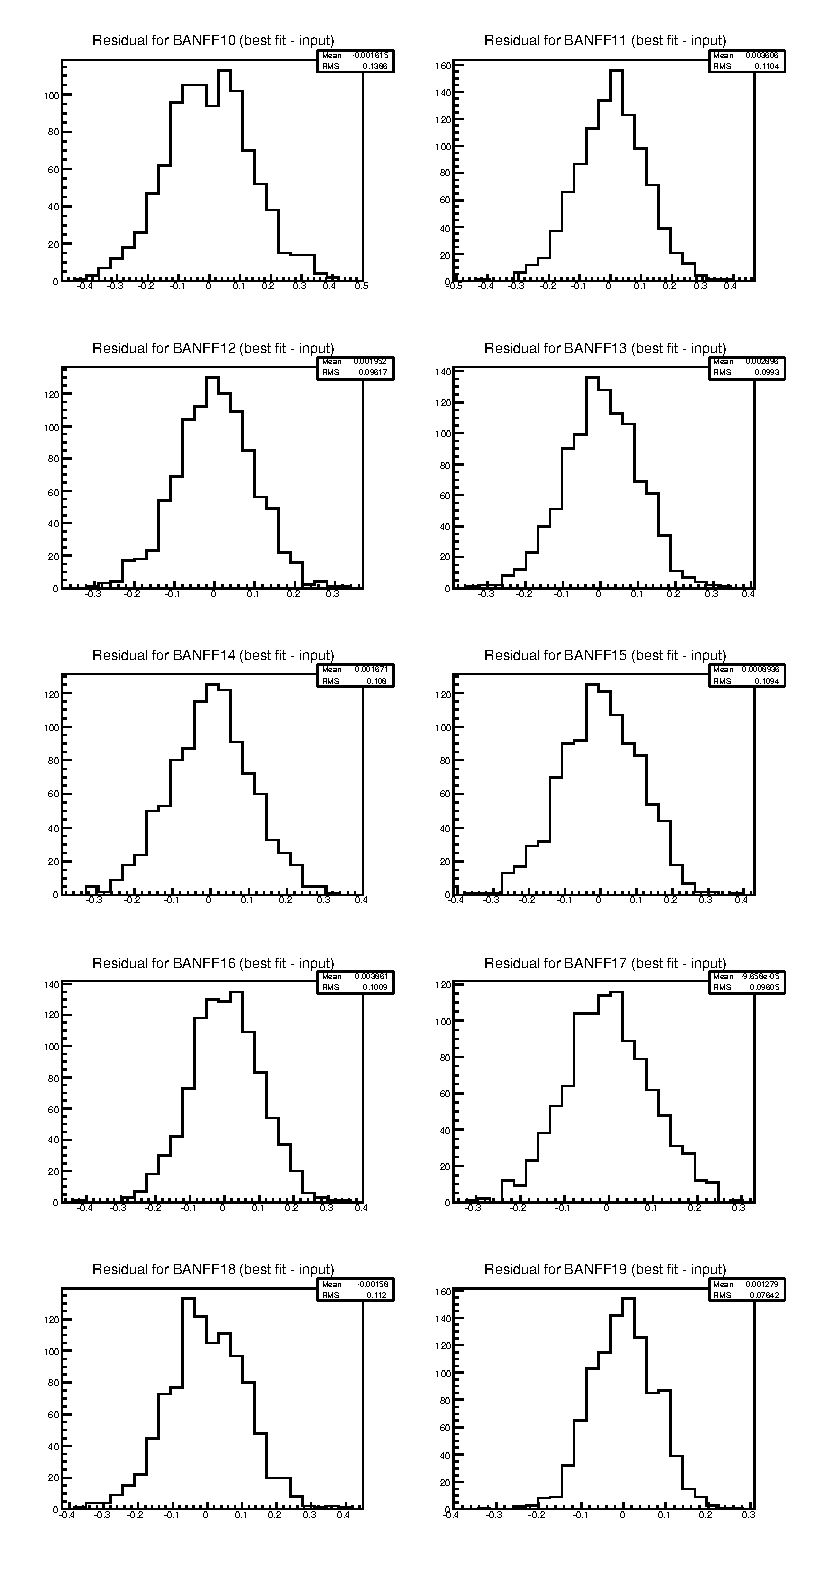
\includegraphics[width=25pc]{images/appendix/fitter_performance/Syst2_residuals_joint_syst_point0.eps}
\caption{
	Distribution of residuals of the BANFF (10-19) systematic parameters in the '4 + 83' fit for oscillation point \# 0. 
 }
\end{figure*}

\begin{figure*}[htbc]	
\center
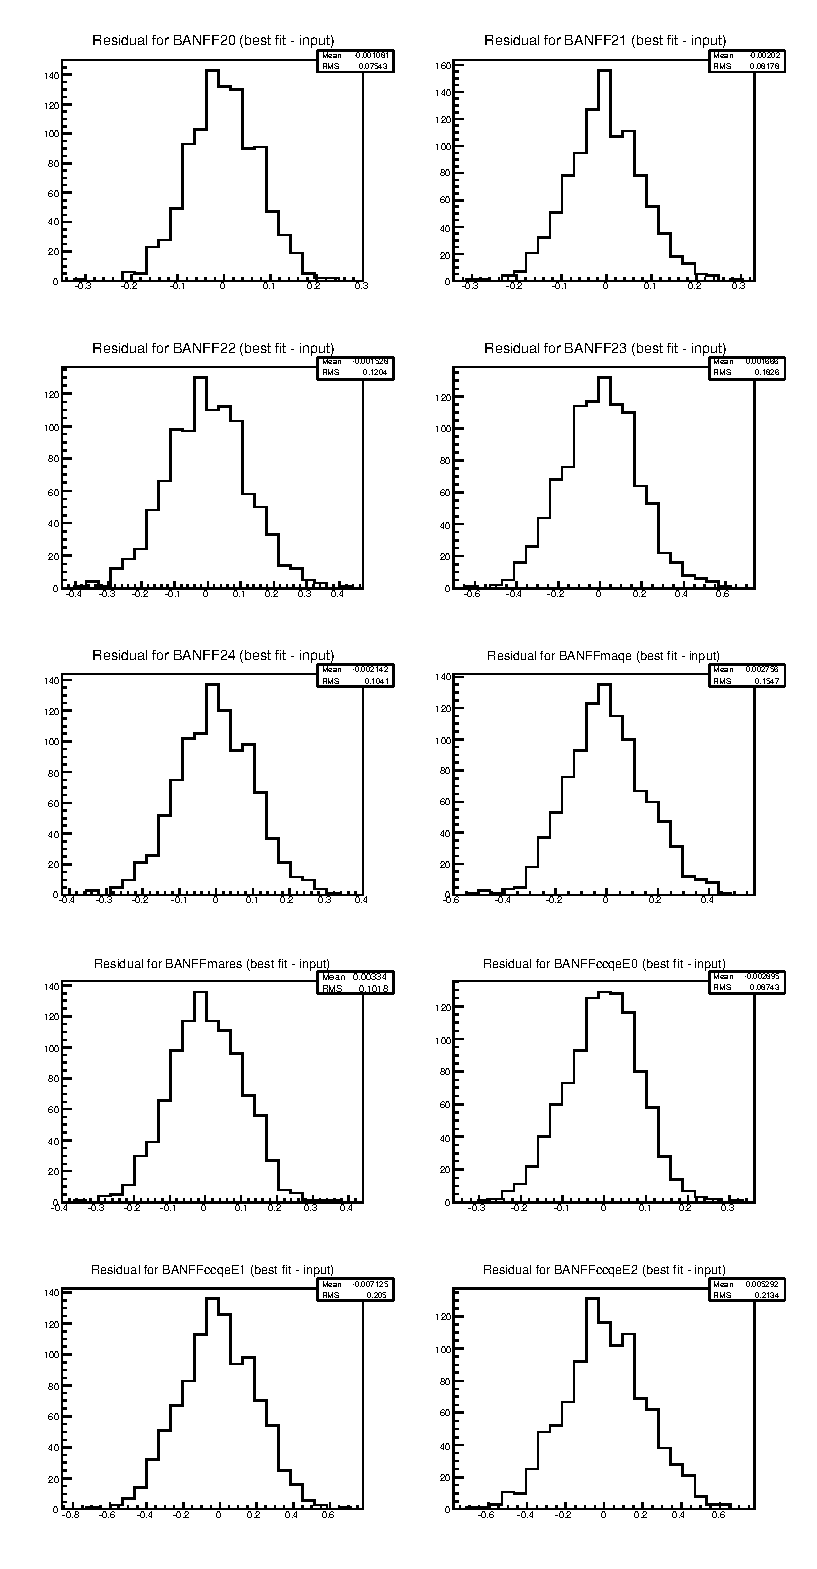
\includegraphics[width=25pc]{images/appendix/fitter_performance/Syst3_residuals_joint_syst_point0.eps}
\caption{
	Distribution of residuals of the  BANFF (20-29) systematic parameters in the '4 + 83' fit for oscillation point \# 0. 
 }
\end{figure*}

\begin{figure*}[htbc]	
\center
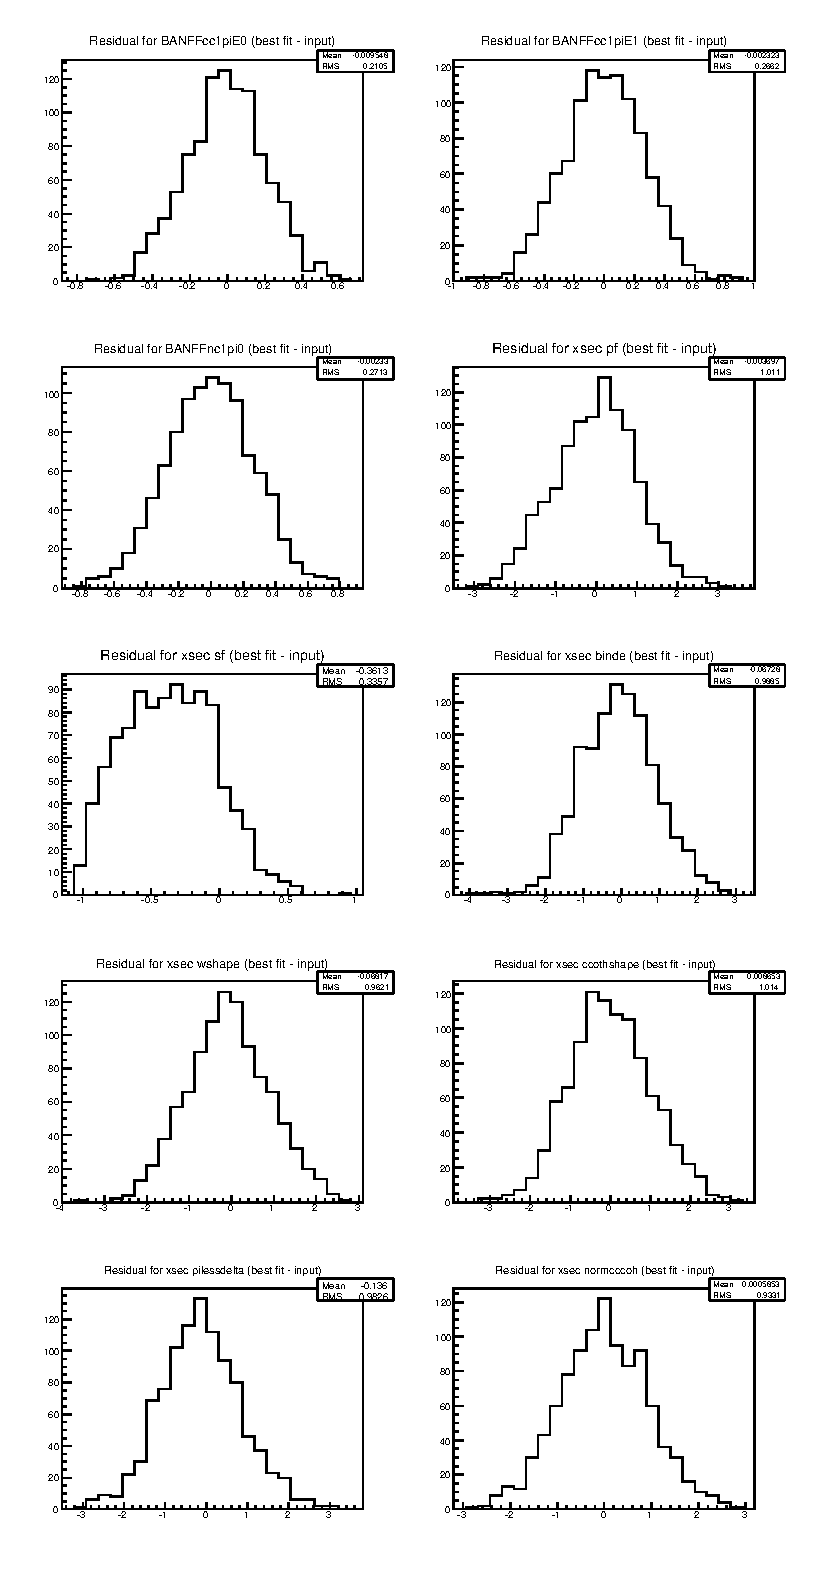
\includegraphics[width=25pc]{images/appendix/fitter_performance/Syst4_residuals_joint_syst_point0.eps}
\caption{
	Distribution of residuals of the BANFF (30-32) and uncorrelated cross sections (I) systematic parameters in the '4 + 83' fit for oscillation point \# 0. 
 }
\end{figure*}

\begin{figure*}[htbc]	
\center
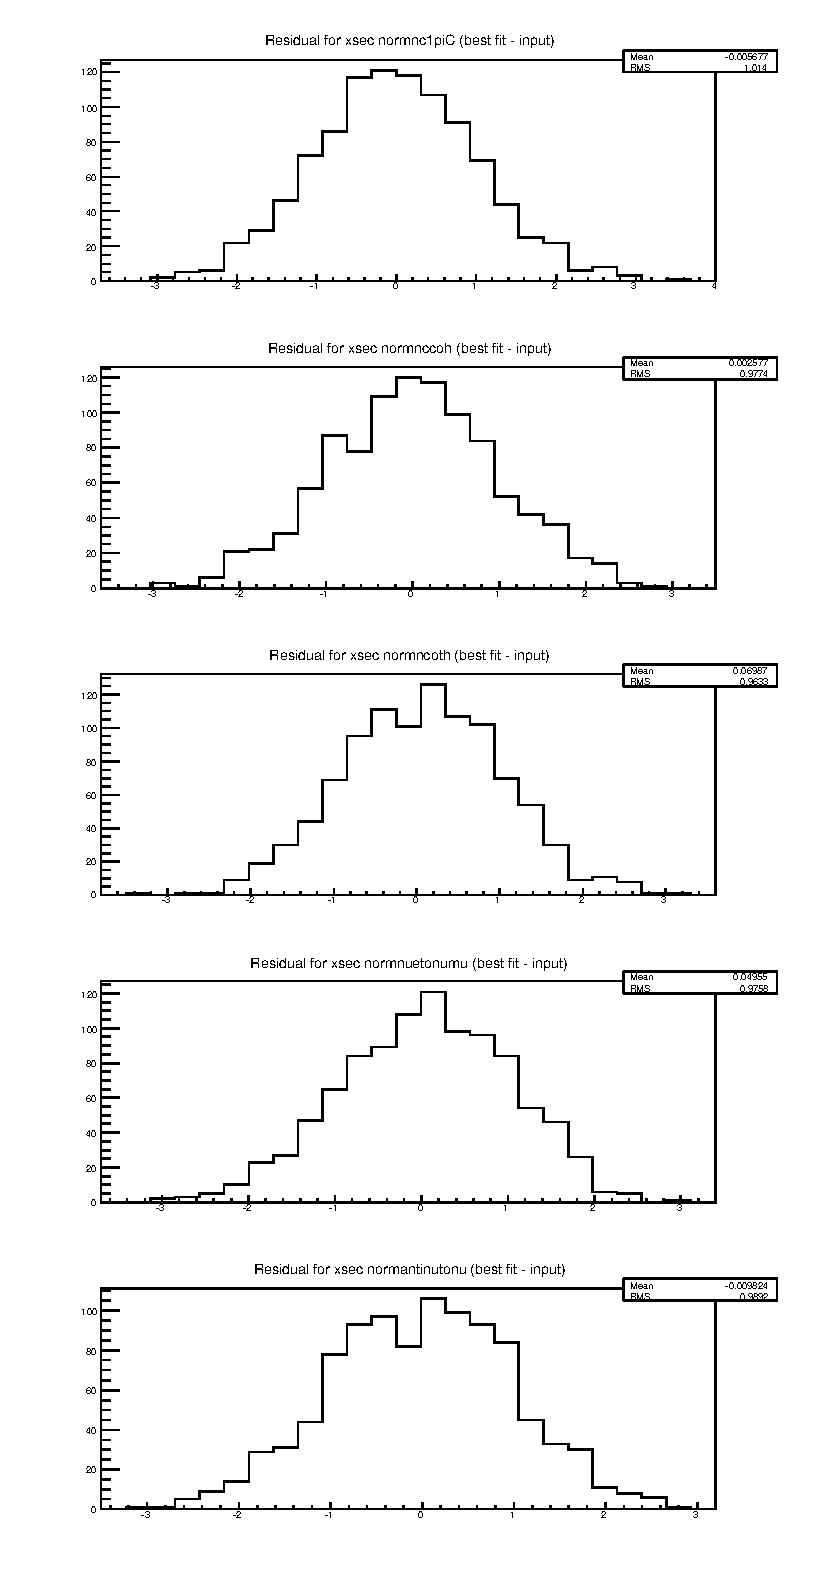
\includegraphics[width=20pc]{images/appendix/fitter_performance/Syst5_residuals_joint_syst_point0.eps}
\caption{
	Distribution of residuals of uncorrelated cross sections (II) systematic parameters in the '4 + 83' fit for oscillation point \# 0. 
 }
\end{figure*}


\begin{figure*}[htbc]	
\center
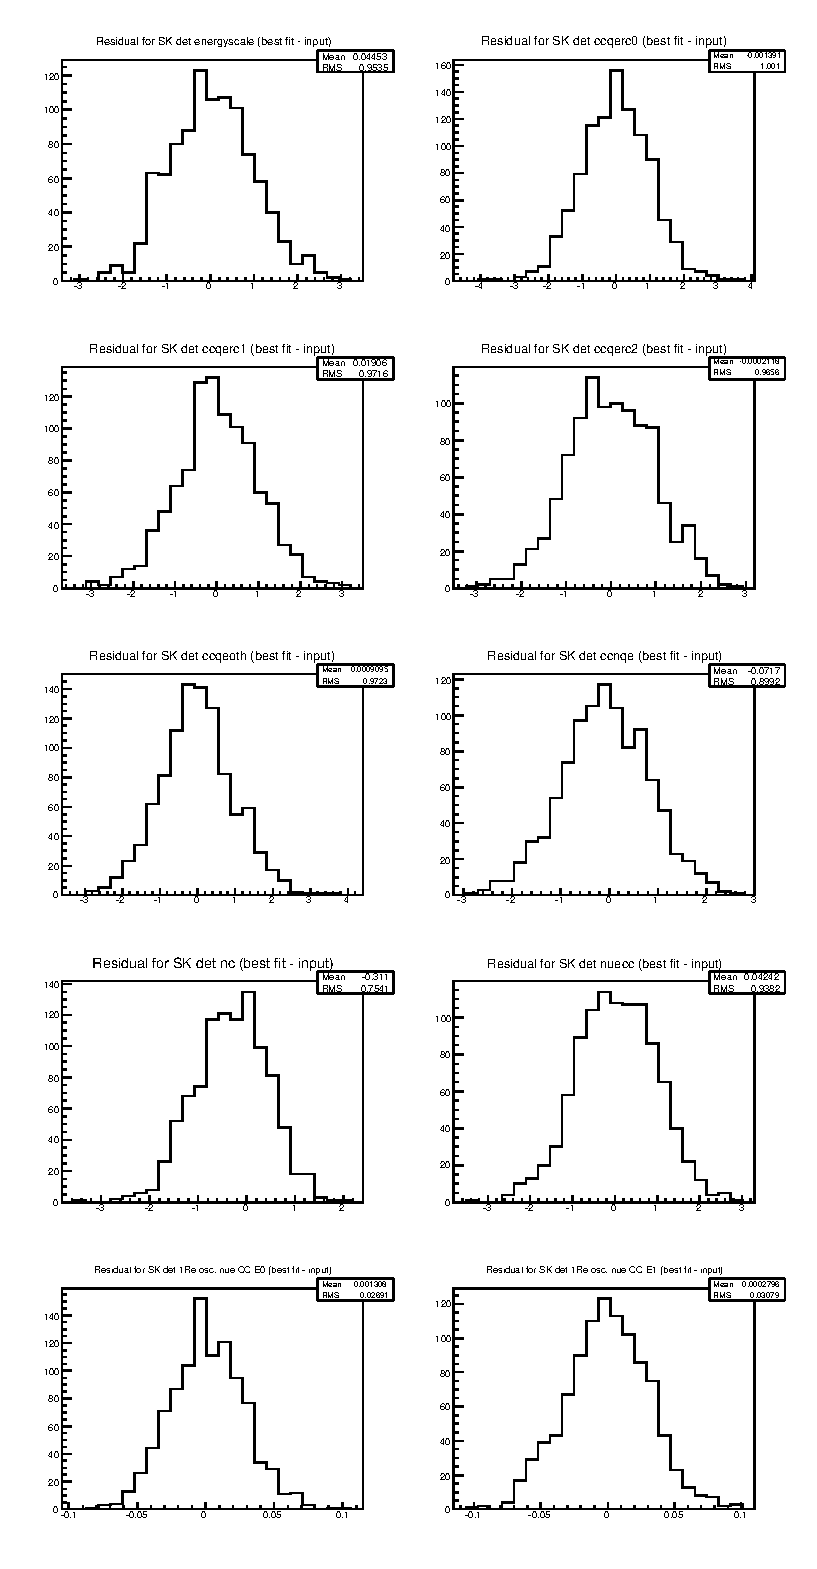
\includegraphics[width=25pc]{images/appendix/fitter_performance/Syst6_residuals_joint_syst_point0.eps}
\caption{
	Distribution of residuals of SK detector (I) systematic parameters in the '4 + 83' fit for oscillation point \# 0. 
 }
\end{figure*}


\begin{figure*}[htbc]	
\center
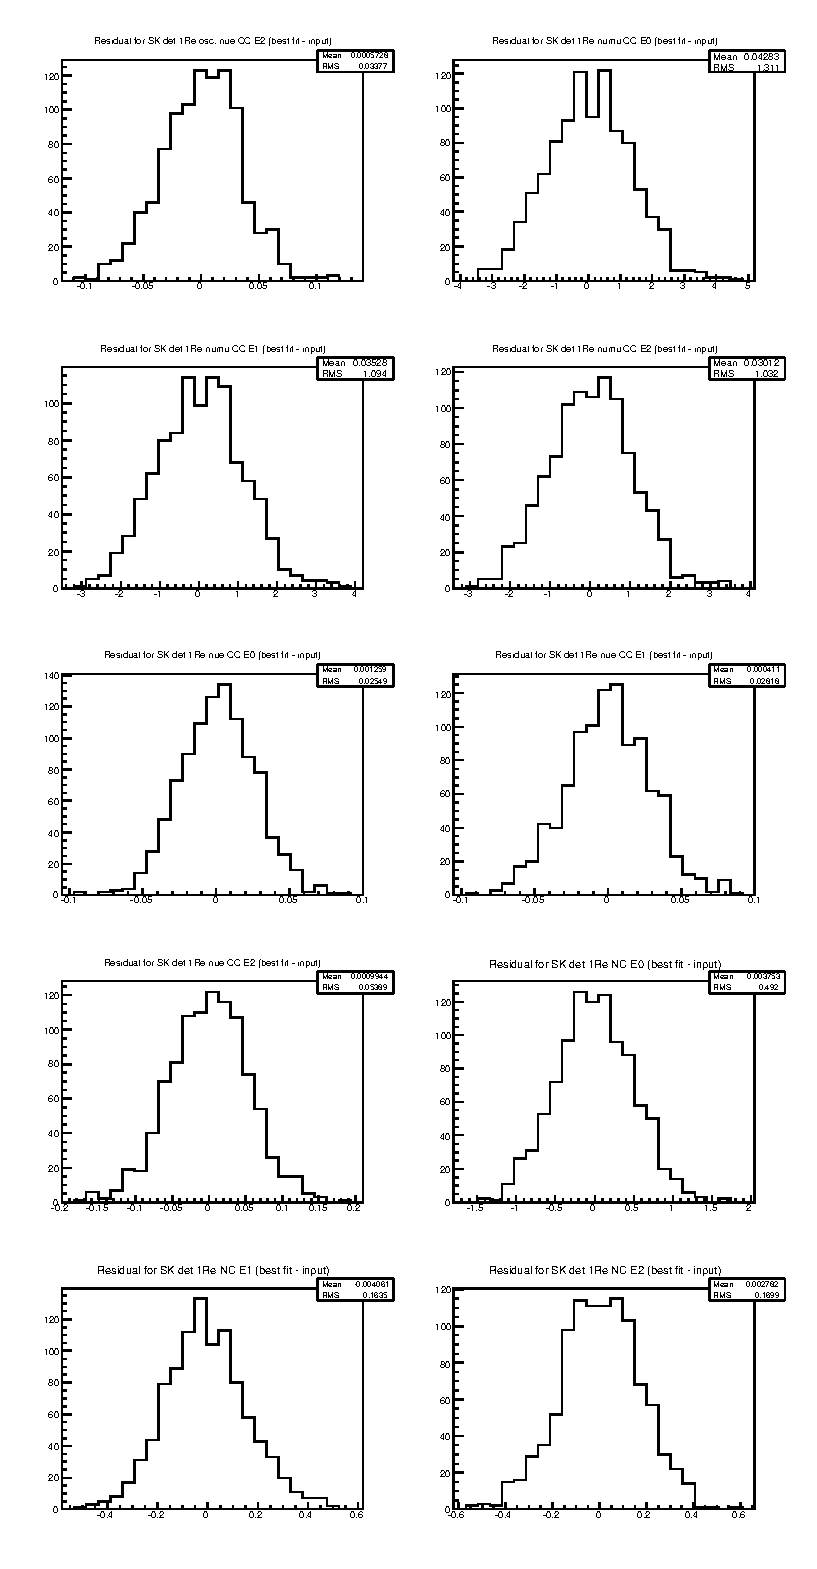
\includegraphics[width=25pc]{images/appendix/fitter_performance/Syst7_residuals_joint_syst_point0.eps}
\caption{
	Distribution of residuals of SK detector (II) systematic parameters in the '4 + 83' fit for oscillation point \# 0. 
 }
\end{figure*}

\begin{figure*}[htbc]	
\center
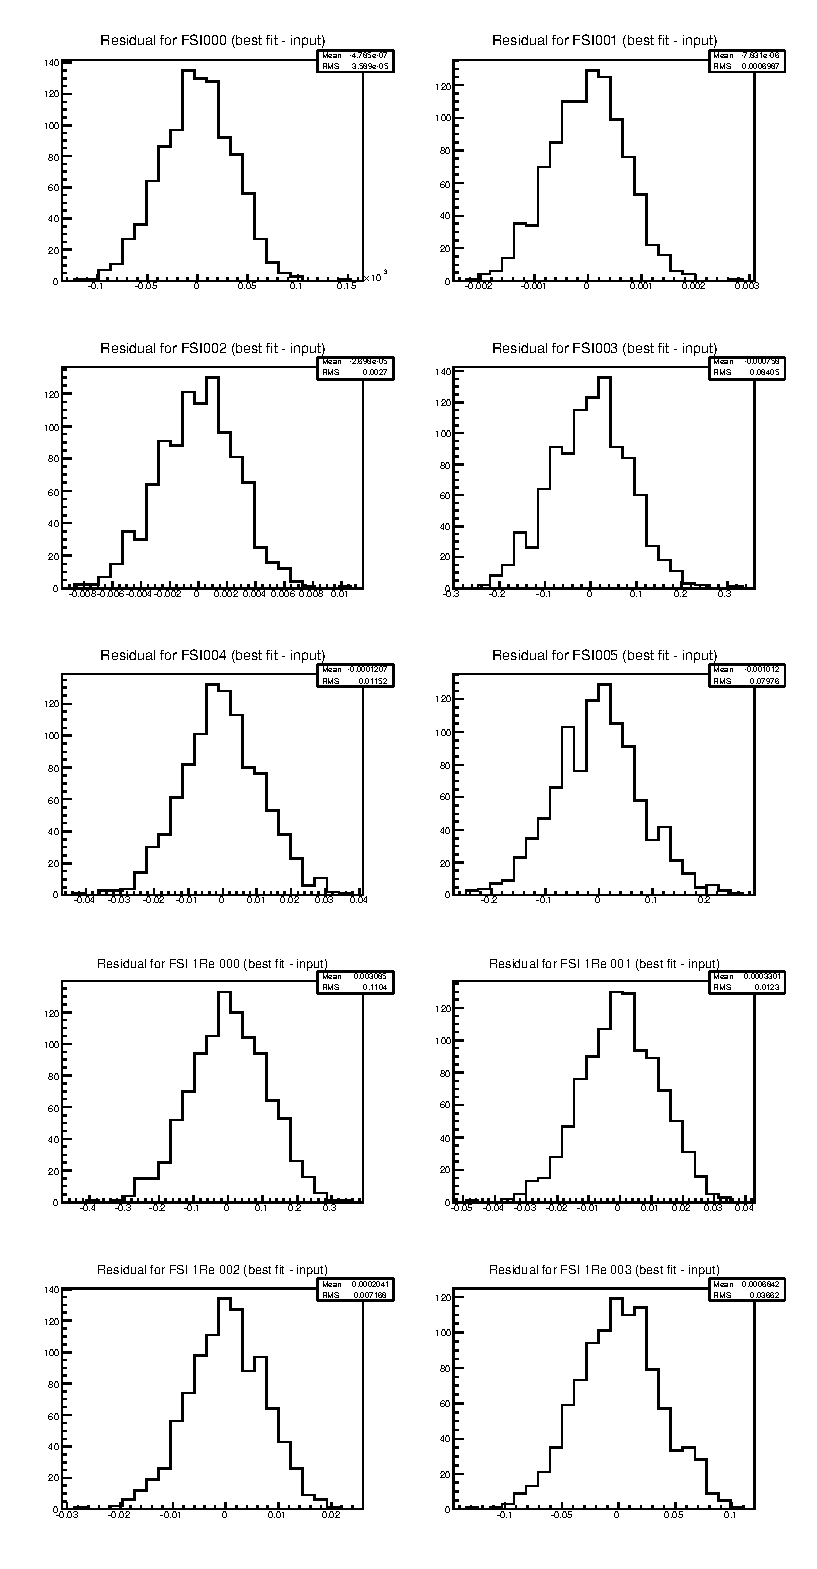
\includegraphics[width=25pc]{images/appendix/fitter_performance/Syst8_residuals_joint_syst_point0.eps}
\caption{
	Distribution of residuals of FSI+SI (I) systematic parameters in the '4 + 83' fit for oscillation point \# 0. 
 }
\end{figure*}

\begin{figure*}[htbc]	
\center
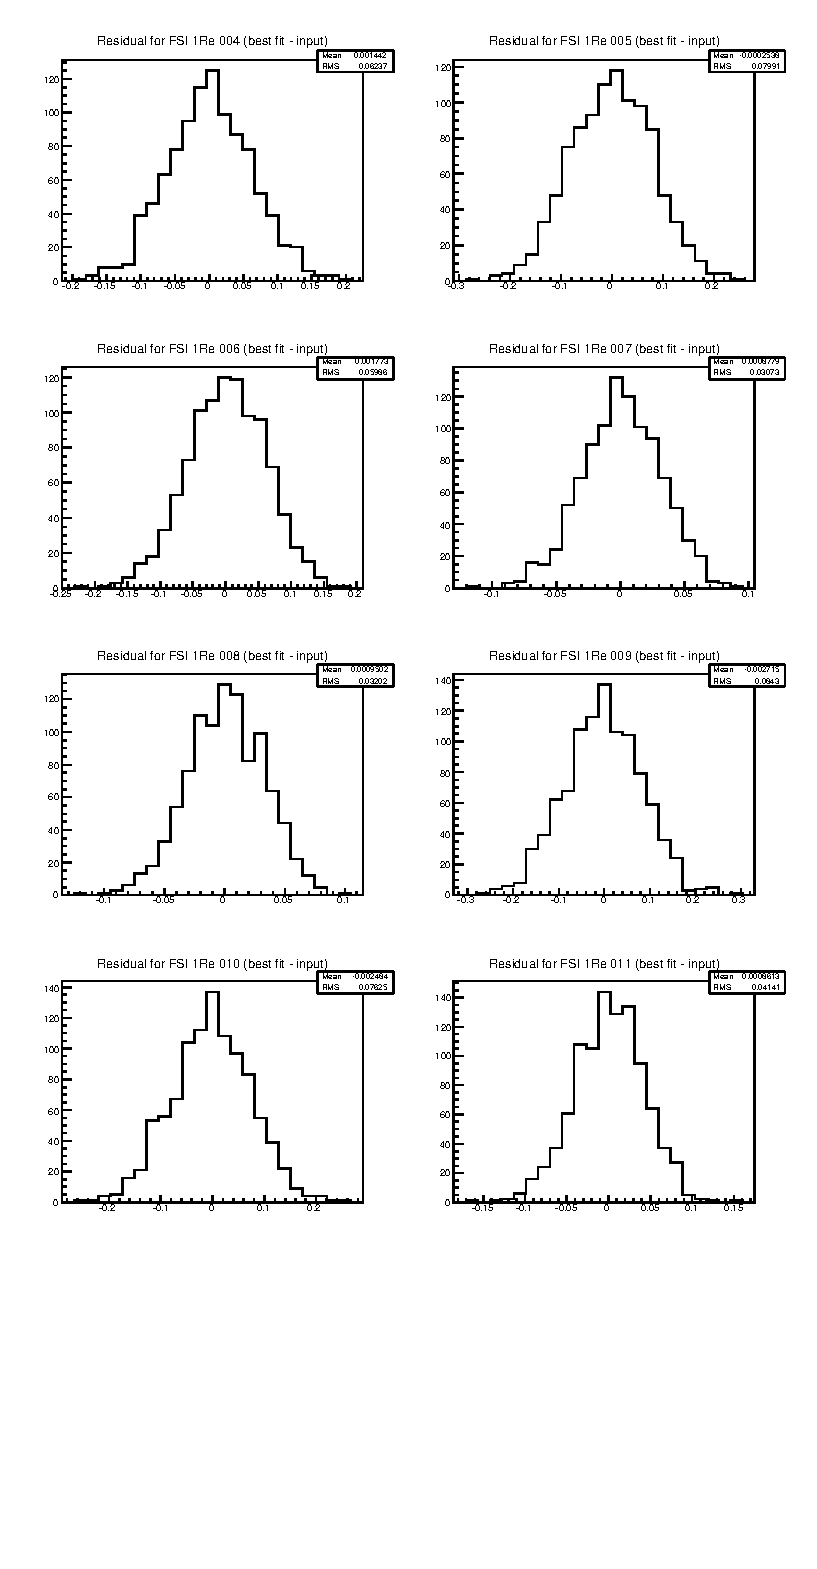
\includegraphics[width=25pc]{images/appendix/fitter_performance/Syst9_residuals_joint_syst_point0.eps}
\caption{
	Distribution of residuals of FSI+SI (I) systematic parameters in the '4 + 83' fit for oscillation point \# 0. 
 }
 \label{fig:residuals_483_syst_last}
\end{figure*}






%%% SUMMARIES

\clearpage

\begin{figure*}[htb]	
\begin{minipage}[t]{0.5\linewidth}
\center
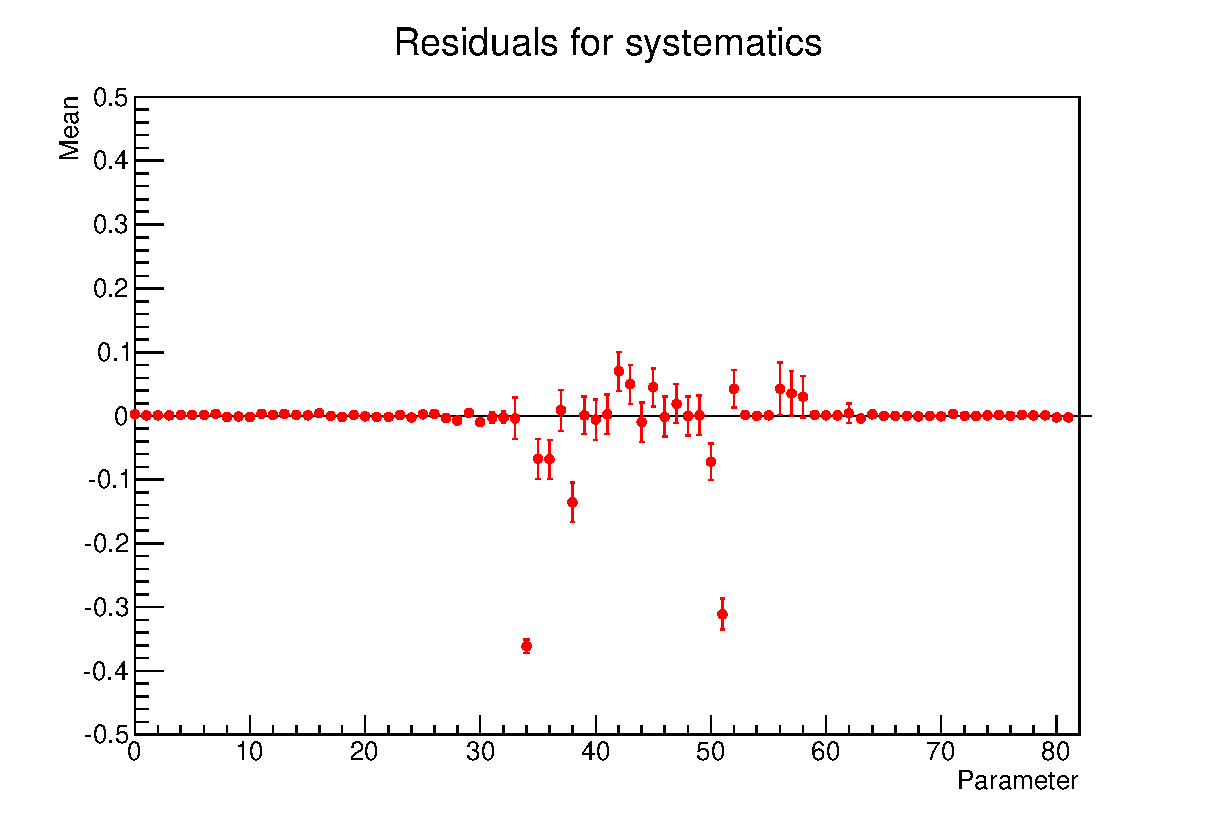
\includegraphics[width=20pc]{images/appendix/fitter_performance/Summary_residuals_joint_syst_point0.eps}
\caption{
	Summary of distribution of residuals of systematic parameters in the '4 + 83' fit for oscillation point \# 0. 
 }
 \label{fig:systematics_point0}
 \end{minipage}
\hspace{0.02\linewidth}	
 \begin{minipage}[t]{0.5\linewidth}
\center
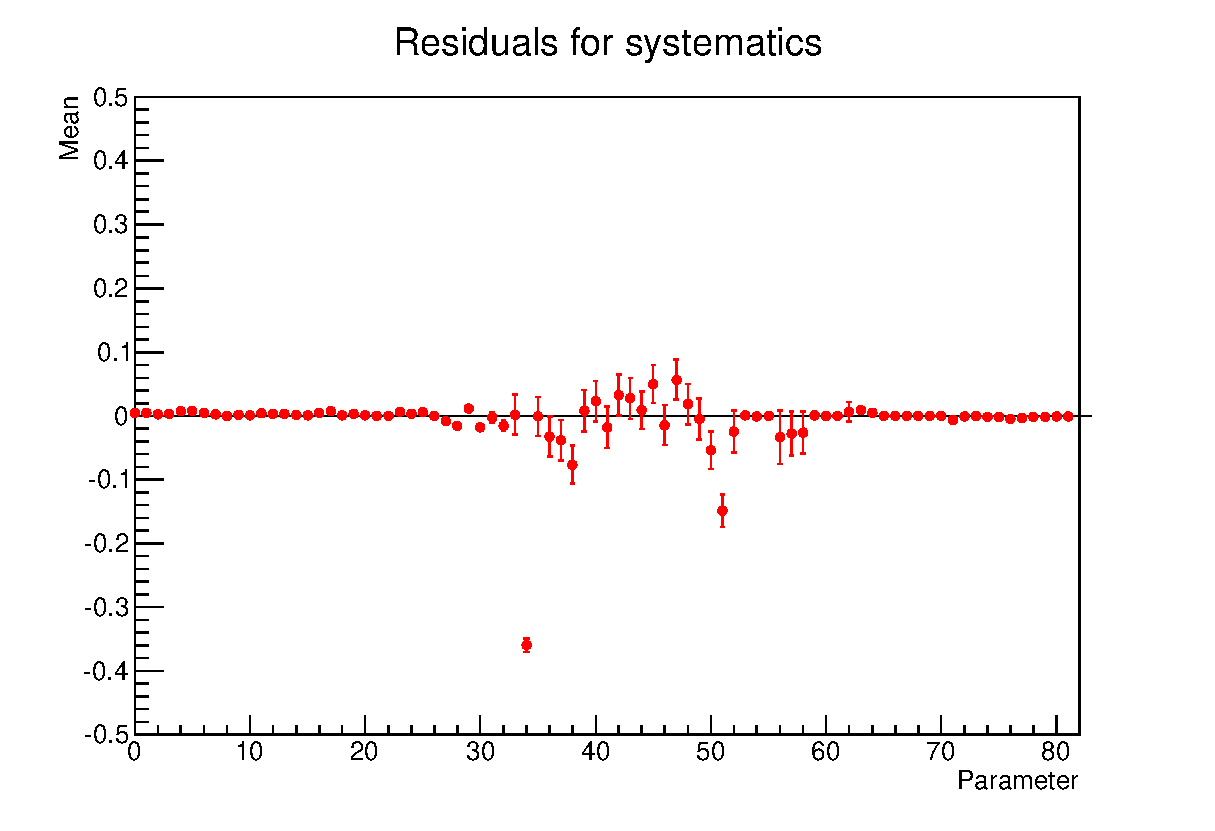
\includegraphics[width=20pc]{images/appendix/fitter_performance/Summary_residuals_joint_syst_point1.eps}
\caption{
	Summary of distribution of residuals of systematic parameters in the '4 + 83' fit for oscillation point \# 1. 
 }
 \end{minipage}

\end{figure*}



\begin{figure*}[htb]	
\begin{minipage}[t]{0.5\linewidth}
\center
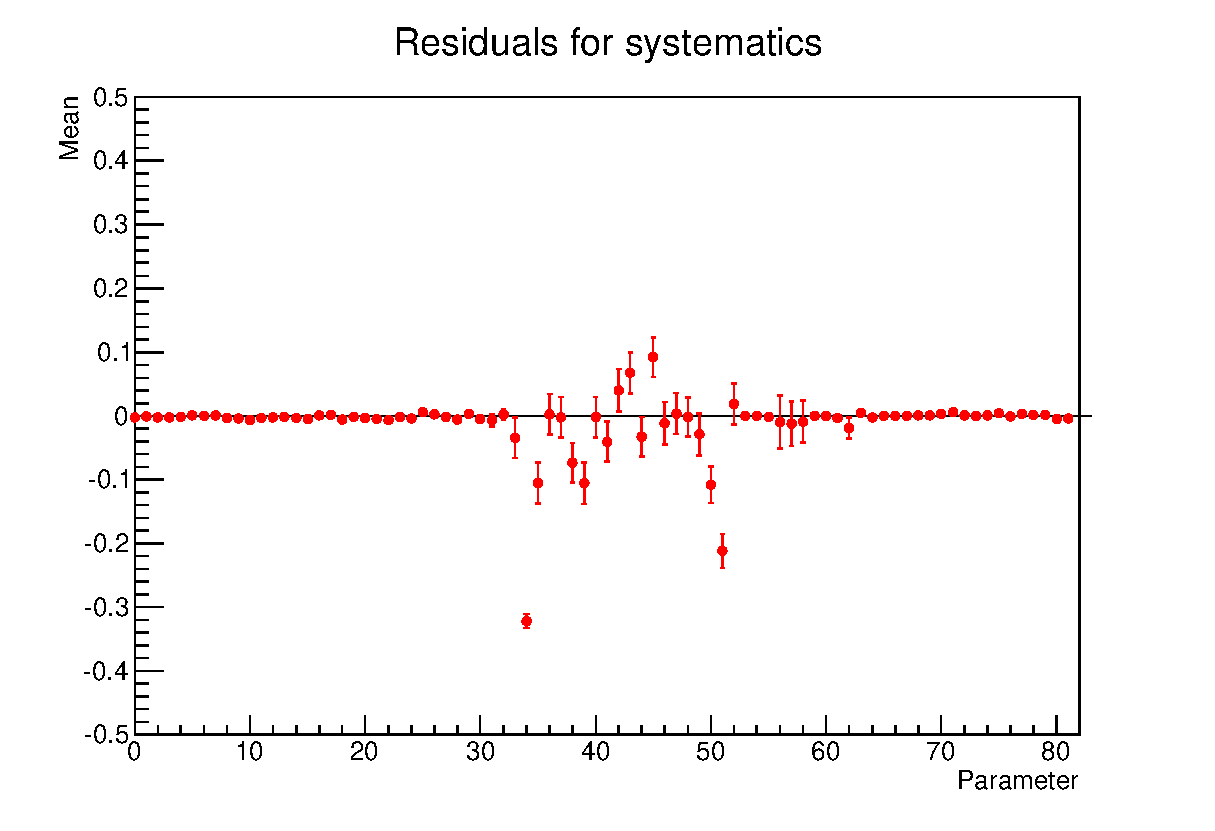
\includegraphics[width=20pc]{images/appendix/fitter_performance/Summary_residuals_joint_syst_point2.eps}
\caption{
	Summary of distribution of residuals of systematic parameters in the '4 + 83' fit for oscillation point \# 2. 
 }
 \label{fig:systematics_point2}
 \end{minipage}
\hspace{0.02\linewidth}	
 \begin{minipage}[t]{0.5\linewidth}
\center
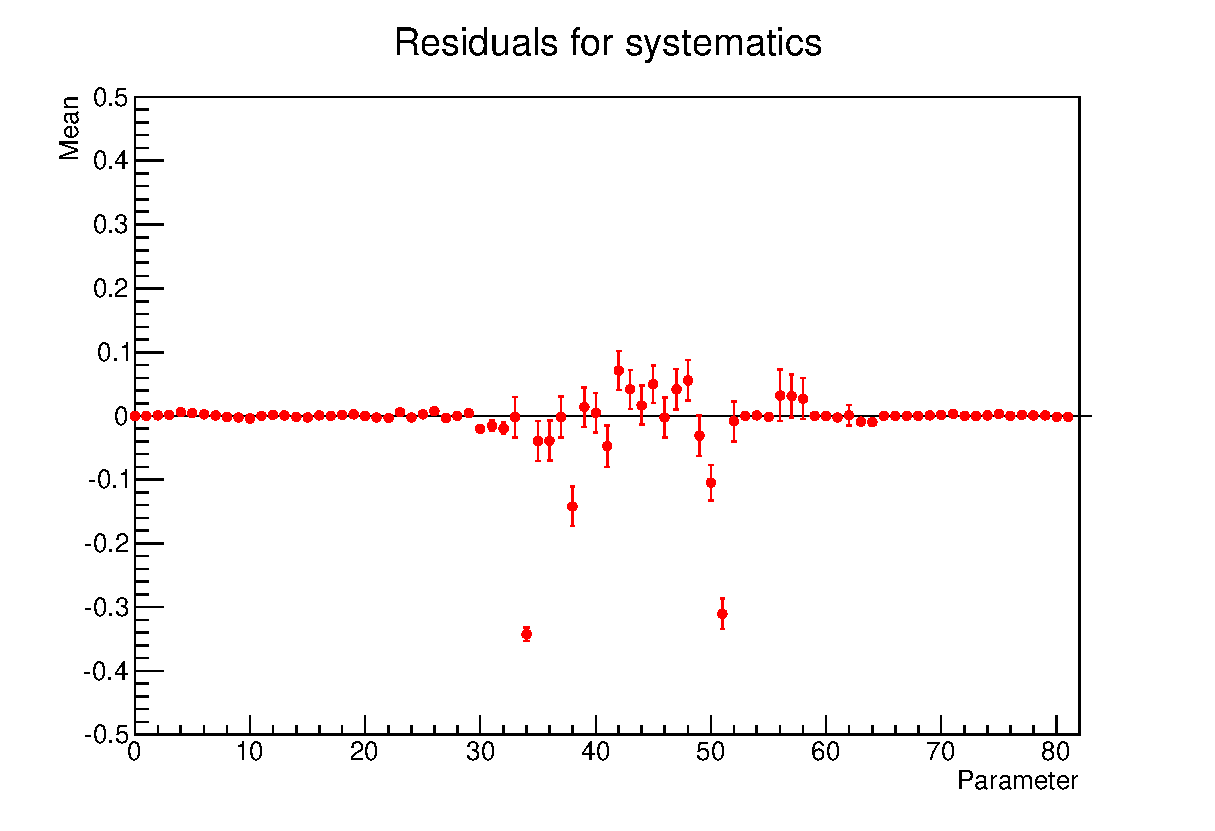
\includegraphics[width=20pc]{images/appendix/fitter_performance/Summary_residuals_joint_syst_point3.eps}
\caption{
	Summary of distribution of residuals of systematic parameters in the '4 + 83' fit for oscillation point \# 3. 
 }
 \end{minipage}

\end{figure*}


\begin{figure*}[htb]	
\begin{minipage}[t]{0.5\linewidth}
\center
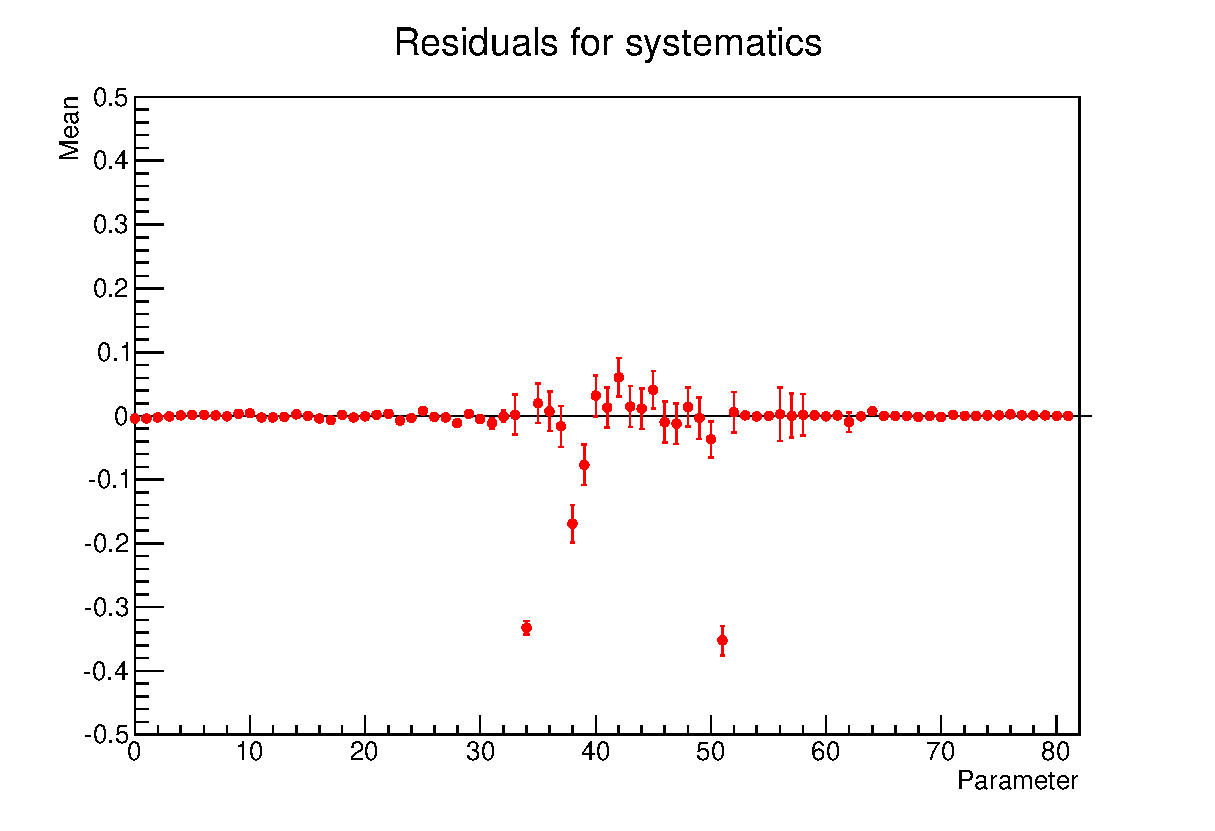
\includegraphics[width=20pc]{images/appendix/fitter_performance/Summary_residuals_joint_syst_point4.eps}
\caption{
	Summary of distribution of residuals of systematic parameters in the '4 + 83' fit for oscillation point \# 4. 
 }
 \label{fig:systematics_point4}
 \end{minipage}
\hspace{0.02\linewidth}	
 \begin{minipage}[t]{0.5\linewidth}
\center
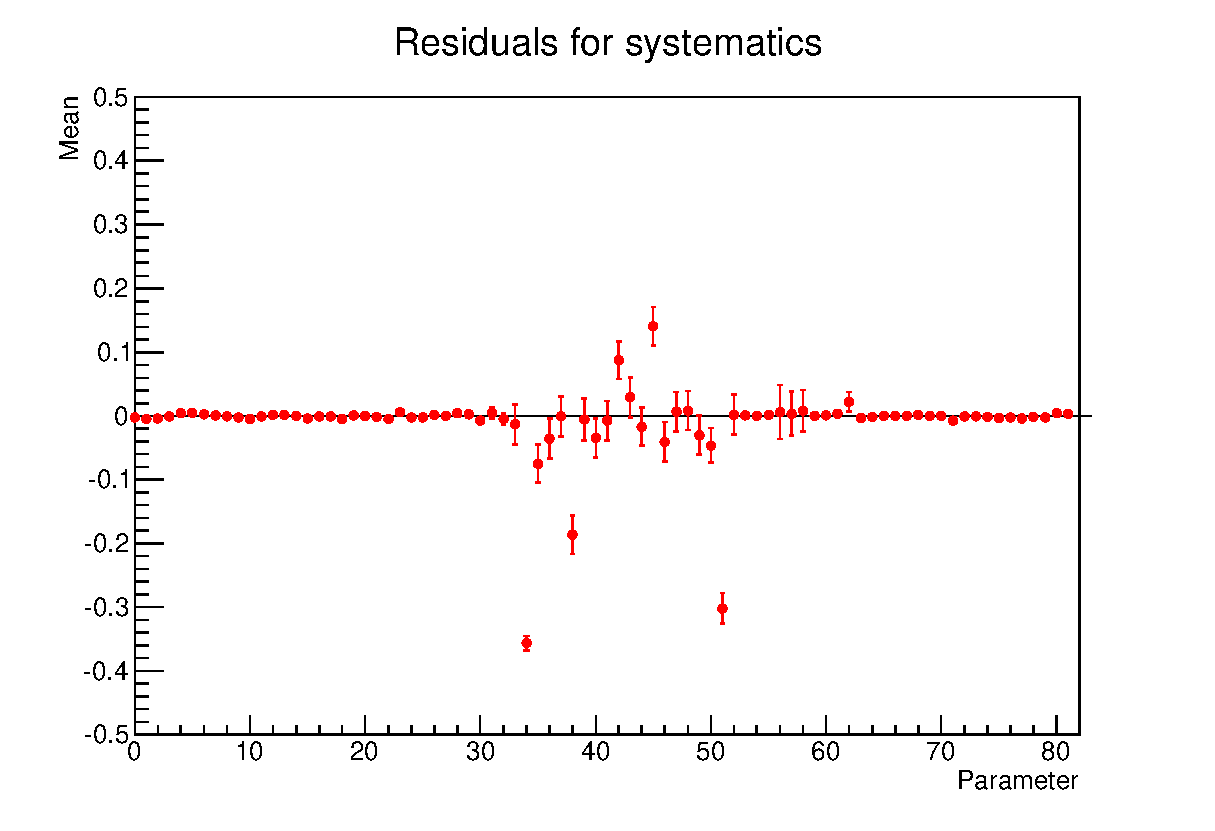
\includegraphics[width=20pc]{images/appendix/fitter_performance/Summary_residuals_joint_syst_point5.eps}
\caption{
	Summary of distribution of residuals of systematic parameters in the '4 + 83' fit for oscillation point \# 5. 
 }
 \end{minipage}

\end{figure*}


\begin{figure*}[htb]	
\begin{minipage}[t]{0.5\linewidth}
\center
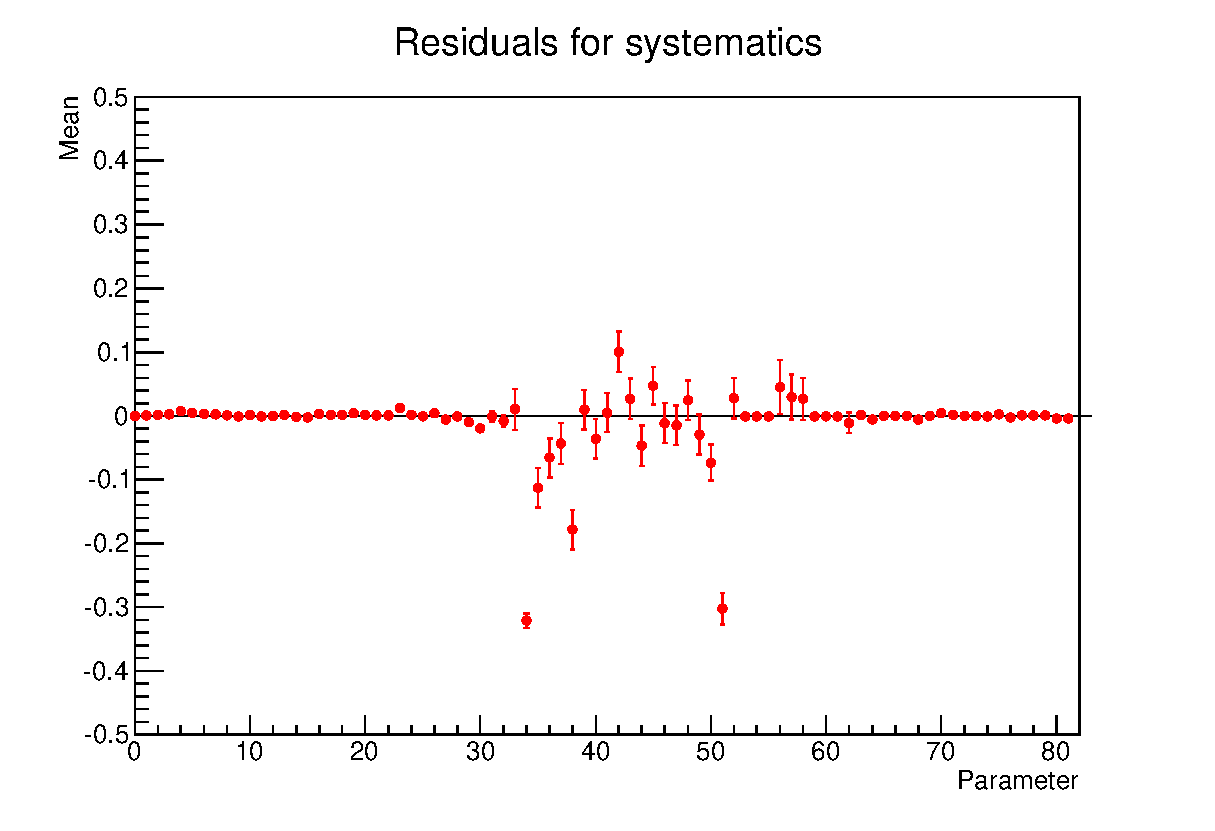
\includegraphics[width=20pc]{images/appendix/fitter_performance/Summary_residuals_joint_syst_point6.eps}
\caption{
	Summary of distribution of residuals of systematic parameters in the '4 + 83' fit for oscillation point \# 6. 
 }
 \label{fig:systematics_point6}
 \end{minipage}
\hspace{0.02\linewidth}	
 \begin{minipage}[t]{0.5\linewidth}
\center
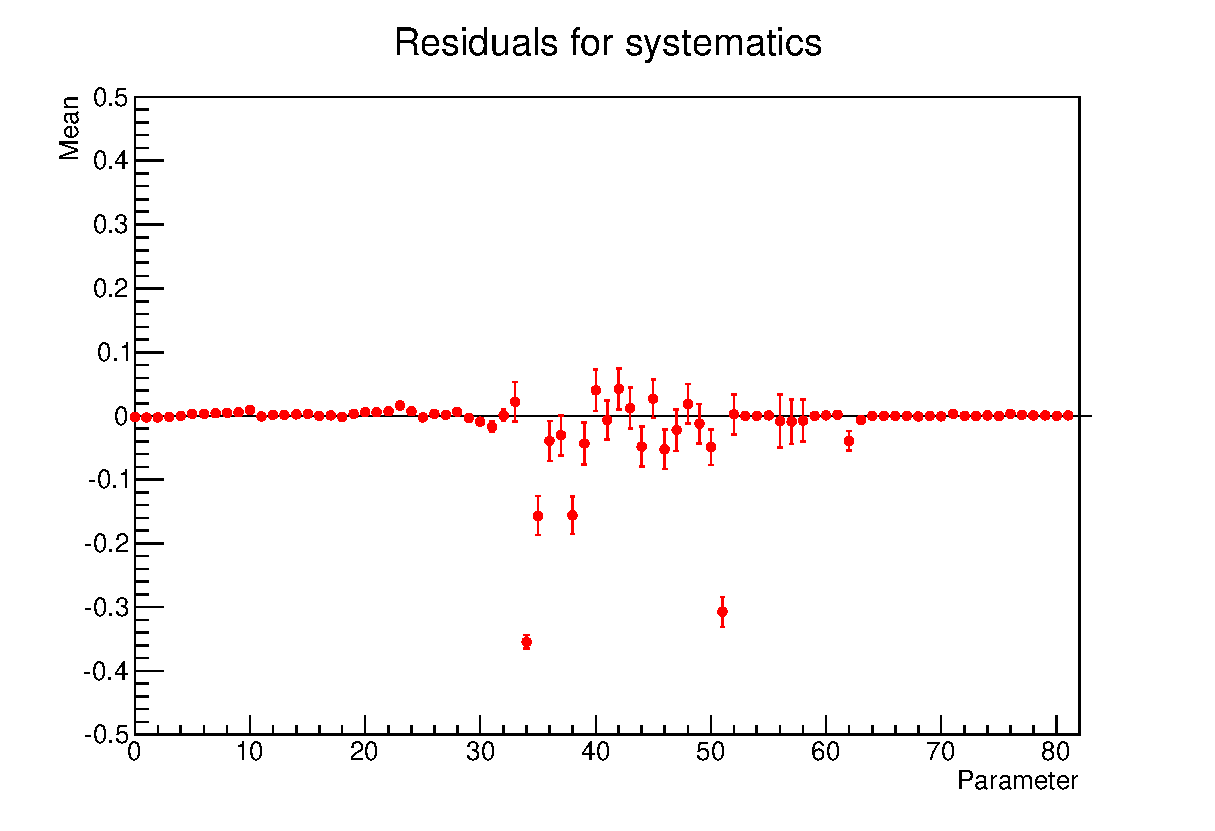
\includegraphics[width=20pc]{images/appendix/fitter_performance/Summary_residuals_joint_syst_point7.eps}
\caption{
	Summary of distribution of residuals of systematic parameters in the '4 + 83' fit for oscillation point \# 7. 
 }
 \end{minipage}

\end{figure*}


\begin{figure*}[htb]	
\begin{minipage}[t]{0.5\linewidth}
\center
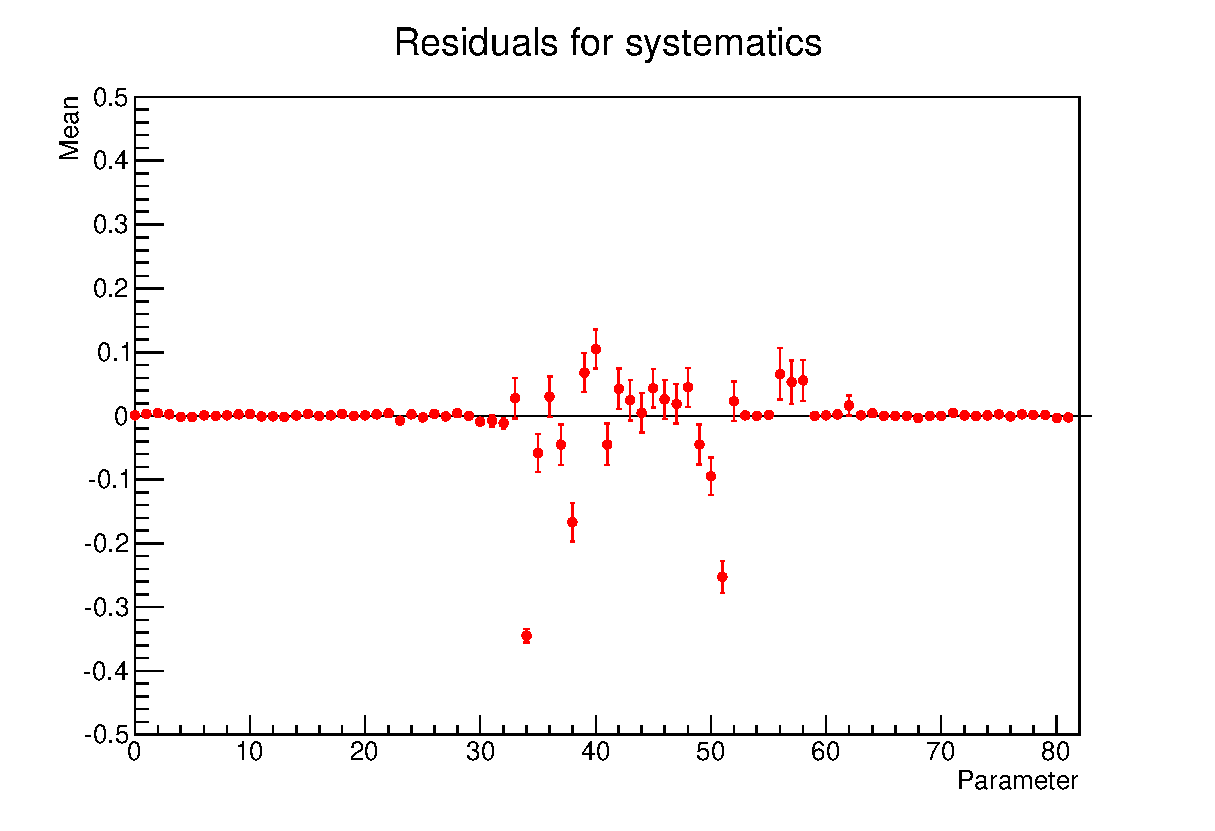
\includegraphics[width=20pc]{images/appendix/fitter_performance/Summary_residuals_joint_syst_point8.eps}
\caption{
	Summary of distribution of residuals of systematic parameters in the '4 + 83' fit for oscillation point \# 8. 
 }
 \label{fig:systematics_point8}
 \end{minipage}
\hspace{0.02\linewidth}	
 \begin{minipage}[t]{0.5\linewidth}
\center
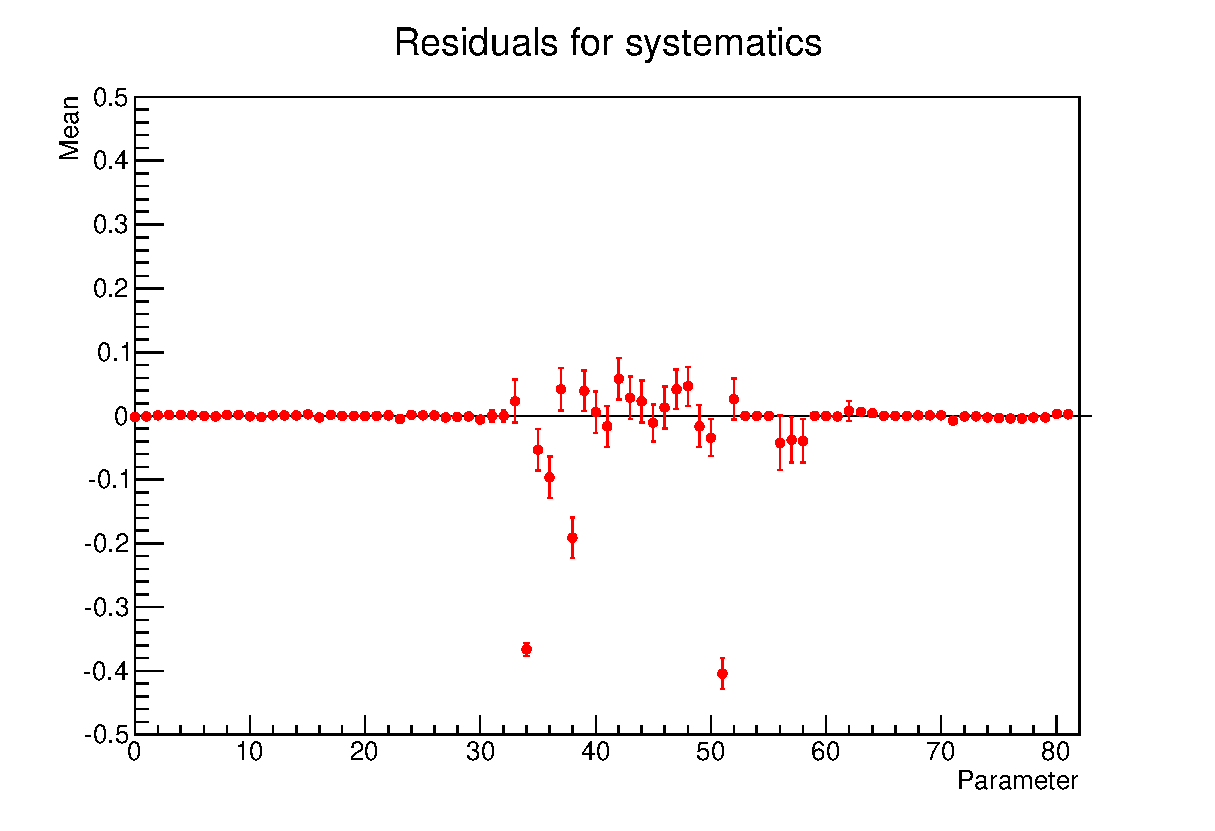
\includegraphics[width=20pc]{images/appendix/fitter_performance/Summary_residuals_joint_syst_point9.eps}
\caption{
	Summary of distribution of residuals of systematic parameters in the '4 + 83' fit for oscillation point \# 9. 
 }
 \end{minipage}
 \label{fig:systematics_point9}
\end{figure*}

